%% 
%% Copyright 2007-2024 Elsevier Ltd
%% 
%% This file is part of the 'Elsarticle Bundle'.
%% ---------------------------------------------
%% 
%% It may be distributed under the conditions of the LaTeX Project Public
%% License, either version 1.3 of this license or (at your option) any
%% later version.  The latest version of this license is in
%%    http://www.latex-project.org/lppl.txt
%% and version 1.3 or later is part of all distributions of LaTeX
%% version 1999/12/01 or later.
%% 
%% The list of all files belonging to the 'Elsarticle Bundle' is
%% given in the file `manifest.txt'.
%% 
%% Template article for Elsevier's document class `elsarticle'
%% with numbered style bibliographic references
%% SP 2008/03/01
%% $Id: elsarticle-template-num.tex 249 2024-04-06 10:51:24Z rishi $
%%
\documentclass[final,10pt]{elsarticle}
\usepackage[margin=1.2in]{geometry}  % 1-inch margins on all sides
\usepackage{lineno}
\usepackage{csquotes}
\usepackage{float}
\usepackage{booktabs}
\usepackage{graphicx}
\usepackage{eurosym}
\usepackage{longtable}
\usepackage{hyperref}
\usepackage{xcolor}
\definecolor{betterblue}{HTML}{669bbc}
\usepackage[defaultcolor=betterblue]{changes}
\usepackage{subcaption}
%\usepackage[printonlyused ]{acronym}
\usepackage{acronym}
%% Use the option review to obtain double line spacing
%% \documentclass[authoryear,preprint,review,12pt]{elsarticle}

%% Use the options 1p,twocolumn; 3p; 3p,twocolumn; 5p; or 5p,twocolumn
%% for a journal layout:
%% \documentclass[final,1p,times]{elsarticle}
%% \documentclass[final,1p,times,twocolumn]{elsarticle}
%% \documentclass[final,3p,times]{elsarticle}
%% \documentclass[final,3p,times,twocolumn]{elsarticle}
%% \documentclass[final,5p,times]{elsarticle}
%% \documentclass[final,5p,times,twocolumn]{elsarticle}

%% For including figures, graphicx.sty has been loaded in
%% elsarticle.cls. If you prefer to use the old commands
%% please give \usepackage{epsfig}

%% The amssymb package provides various useful mathematical symbols
\usepackage{amssymb}
%% The amsmath package provides various useful equation environments.
\usepackage{amsmath}
%% The amsthm package provides extended theorem environments
%% \usepackage{amsthm}

%% The lineno packages adds line numbers. Start line numbering with
%% \begin{linenumbers}, end it with \end{linenumbers}. Or switch it on
%% for the whole article with \linenumbers.
%% \usepackage{lineno}

\journal{Energy}

\begin{document}
% without table print
\acrodef{CCGT}[CCGT]{Combined-cycle gas turbines}
\acrodef{CD}[CD]{charging demand}
\acrodef{CT}[CT]{charging types}
\acrodef{CP}[CP]{charging processes}
\acrodef{DC}[DC]{direct current}
\acrodef{DA}[DA]{day-ahead}
\acrodef{DSM}[DSM]{demand-side management}
\acrodef{EV}[EV]{electric vehicle}
\acrodef{ENTSOE}[ENTSO-E]{European network of transmission system operators}
\acrodef{FBMC}[FBMC]{flow based market coupling}
\acrodef{LP}[LP]{linear programming}
\acrodef{MBCM}[MBCM]{market-based congestion management}
\acrodef{MILP}[MILP]{mixed integer linear programming}
\acrodef{NT}[NT]{National Trends}
\acrodef{NECP}[NECP]{national energy and climate plans}
\acrodef{NSE}[NSE]{not supplied energy}
\acrodef{NTC}[NTC]{net transfer capacities}
\acrodef{OM}[O\&M]{operation and maintenance costs}
\acrodef{PHS}[PHS]{pumped hydro-power storage units}
\acrodef{PTDF}[PTDF]{power transfer distribution factor}
\acrodef{PV}[PV]{photovoltaic}
\acrodef{RESE}[RES-E]{renewable energy sources for electricity}
\acrodef{RoR}[RoR]{run-of-the-river hydroelectricity}
\acrodef{SEW}[SEW]{Socio-economic welfare}
\acrodef{SRMC}[SRMC]{short run marginal costs}
\acrodef{TSO}[TSO]{transmission system operator}
\acrodef{V2G}[V2G]{vehicle-to-grid}
\acrodef{VoLL}[VoLL]{value of lost load}
\acrodef{TSO}[TSO]{transmisison grid operator}
\acrodef{HDT}[HDT]{heavy-duty truck}
\acrodef{LDT}[LDT]{light-duty truck}

\begin{frontmatter}

%% Title, authors and addresses

%% use the tnoteref command within \title for footnotes;
%% use the tnotetext command for theassociated footnote;
%% use the fnref command within \author or \affiliation for footnotes;
%% use the fntext command for theassociated footnote;
%% use the corref command within \author for corresponding author footnotes;
%% use the cortext command for theassociated footnote;
%% use the ead command for the email address,
%% and the form \ead[url] for the home page:
%% \title{Spatial granularity matters: participation ofcommercial electric fleets for redispatch in congested transmission grids\tnoteref{label1}}
%% \tnotetext[label1]{}
%% \author{Name\corref{cor1}\fnref{label2}}
%% \ead{email address}
%% \ead[url]{home page}
%% \fntext[label2]{}
%% \cortext[cor1]{}
%% \affiliation{organization={},
%%             addressline={},
%%             city={},
%%             postcode={},
%%             state={},
%%             country={}}
%% \fntext[label3]{}

% \title{Spatial granularity matters: participation of
% commercial electric vehicle fleets in redispatch in congested
% transmission grids}

\title{The value of flexibility of commercial electric vehicle fleets in the redispatch of congested transmission grids}

%% use optional labels to link authors explicitly to addresses:
\author[label1]{Antonia Golab\footnote{Corresponding author, e-mail: golab@eeg.tuwien.ac.at}}
\author[label1]{Christoph Loschan}
\author[label1,label2]{Sebastian Zwickl-Bernhard}
\author[label1,label2]{Hans Auer}

\affiliation[label1]{organization={Energy Economy Group (EEG), Technische Universität Wien},
            addressline={Gusshausstraße 25-29, E370-3},
            city={Vienna},
            postcode={1040},
            country={Austria}}

\affiliation[label2]{organization={Department of Industrial Economics and Technology Management, The Norwegian University of Science and Technology},
            addressline={Alfred Getz vei 3},
            city={Trondheim},
            postcode={7491},
            country={Norway}}

% \author{Antonia Golab} %% Author name

% %% Author affiliation
% \affiliation{organization={},%Department and Organization
%             addressline={}, 
%             city={},
%             postcode={}, 
%             state={},
%             country={}}

%% Abstract

%% Text of abstract
\begin{abstract}

With the electrification of the transport sector, significant charging loads by the future commercial fleet are expected. The present work aims to give quantitative insight into how impactful the future charging loads of the battery-electric commercial fleet will be to the electricity system. We hereby focus on the day-ahead market and congestion management while applying the proposed modeling framework to the Austrian case with different shares of fleet electrification in 2040. The methodological framework encompasses the spatio-temporal modeling of charging loads as well as optimization models simulating the day-ahead market clearing and the implementation of redispatch measures. Results indicate increased costs for redispatch measures when the flexibility of the aggregated fleet is used in the cost-optimal dispatch. It is demonstrated that the flexibility of the charging processes can be effectively applied in congestion management and reduce redispatch costs by up to 35\%, while optimal charging profiles are observed to vary depending on their geographic allocation.
\end{abstract}



%%Research highlights
\begin{highlights}
\item Future charging profiles for the commercial fleet are modeled.
\item Traffic flow data is used to determine local charging demand.
\item Charging flexibility is used in dispatch and redispatch.
\item The integration of flexibility in the day-ahead market increases grid congestion.
\item Redispatch costs can be effectively decreased by utilizing charging flexibility.

\end{highlights}

%% Keywords
\begin{keyword}
    charging flexibility, commercial fleet charging, battery-electric heavy-duty trucks, congestion management, redispatch 
\end{keyword}

\end{frontmatter}



%% Use \section commands to start a section
\linenumbers  % Start line numbering
\begin{acronym}
    \acro{BEV}{battery-electric vehicle}
    \acro{HDT}{heavy-duty truck}
    \acro{LDT}{light-duty truck}
    \acro{RESE}{renwable energy sources for electricity}
    \acro{TSO}{transmission system operator}

\end{acronym}
\section{Introduction} \label{ref:intro}

    European electricity grid operators are faced with new challenges in the face of the goal of net-zero carbon emissions by the European Union (EU) and the ongoing transition towards a sustainable energy system \cite{european_green_deal, CARLINI201974}. The share of variable and decentralized renewable electricity production has significantly risen during the past two decades \cite{iea_world_energy_statistics}. With this, the amounts of required power for balancing and congestion management of the grid have increased as well \cite{acer_2024_mmr}. 

    Redispatch markets play an intricate part in the congestion management in Central European transmission grids \cite{9221963}. The redispatching of power plants is here performed in cooperation with \aclp{TSO} of neighboring countries. Different ways to reduce the costs of congestion management have been explored in the literature \cite{PILLAY201583} including a wide strand of literature focusing on using the demand-side flexibility of aggregated consumers \cite{GORANSSON2014860}. With the increased electrification in different demand sectors \cite{iea_world_energy_statistics} and increased strengthening of the awareness to participate in electricity markets as a \textit{prosumer} \cite{frieden2020collective}, the range of different potential market participating technologies and concepts to support decentral flexibilities, as well as of required policy frameworks, is becoming wider.

    For the decarbonization in the transport sector, new technologies, as well as the shift to different modes, are important levers discussed in the \textit{Smart Mobility Strategy} paper by the EU \cite{eu_mobility_strategy}. In the road transport sector, the direct electrification of vehicle drive-trains is supported by literature to be the most cost-effective and efficient measure to defossilize the sector on a large scale \cite{Auer2020, Plötz2022}. The introduction of this new technology is connected to requirements in structural changes, such as the deployment of charging infrastructure, as well as changes in logistic processes and travel behavior \cite{LEBROUHI2021103273}. This is particularly a challenge for commercial vehicles, such as trucks and busses \cite{KONSTANTINOU2023100746}. This electrification comes with a significant additional electricity demand but also provides demand-side flexibility \cite{ag2022flexibility}. 
    
    The core objective of this paper is to study the impact of future charging loads of commercial \ac{BEV} fleets on the development of redispatch costs and the potential to use its flexibility to participate in the redispatch market. We hereby apply the case study data for Austria.  First, the spatio-temporal distribution of charging demand and charging capacities is modeled. Second, the charging profiles and flexibility potentials are used to simulate the integration of the flexibility\footnote{In this work, we exclusively consider unidirectional grid-to-vehicle power flow and do not study bidirectional vehicle-to-grid technology as the implementation of the latter is faced with significantly more technical and regulatory challenges \cite{LEBROUHI2021103273}.} of the commercial fleet in the day-ahead market and in congestion management. 
    
    In this context, we address the following three research questions:
        \begin{itemize}
        \item What is the expected charging demand of the commercial \ac{BEV} fleet spatio-temporally distributed in Austria in 2040?
        \item How does the charging and the utilization of the aggregated commercial \ac{BEV} fleet in the day-ahead market and in redispatch measures affect costs for redispatch measures?
        \item How are the charging processes of the commercial \ac{BEV} fleets affected by the central aggregation and flexibility utilization in the day-ahead market and in redispatch measures? 

    \end{itemize}  


%% Use \subsection commands to start a subsection.

\section{Literature review}
    \subsection{Electrification and charging of the commercial fleet}
        Currently, the electrification of the commercial fleet is in significantly earlier stages than the private passenger vehicle sector. One early and significant adopter in the commercial fleet sector is the \ac{LDT} which makes up 89\% of the Austrian commercial fleet \cite{statistik_at_kfz_bestand}. When it comes to the requirements for battery size and charging power, this type of vehicle is comparable to the passenger \ac{BEV}. Other commercial vehicle types that are used for heavy duty require bigger battery capacities due to higher specific energy consumption and longer trip ranges. To overcome this, overhead lines have been used to power electric buses; for example, trolley buses have been in operation in urban applications in some European cities since around the mid of last century \cite{ietmeishner}. Due to difficulties in the social acceptance of installing new overhead lines, the adoption of electric buses that are exclusively battery-powered is becoming the most common in the electrification of city bus fleets.  Electric buses of the latter kind are already in operation on routes matching the driving range of currently available bus models \cite{orf2023}. Moreover, short-haul applications of heavy-duty trucks are projected to be adopted soon\cite{NOLL2022118079}. 

        In the report by \citeauthor{Scherrer2024Requirements}, the authors describe existing barriers to the technology switch to battery-powered medium- and heavy-duty trucks for fleet operators in Germany \cite{Scherrer2024Requirements}. The major barriers refer to the challenges in the deployment of high-power-level charging infrastructure and, moreover, to the difficulty of adopting operational patterns to the need for being flexible in the timing and location of the charging process. This kind of flexibility is especially needed because of the unpredictability of the availability and performance of public charging infrastructure. Given this, extensive research is dedicated to the optimal integration of the charging process in operational schedules. This encompasses the geographic allocation of charging stations and the determination of optimal timing and position of the charging process, as well as the optimization of the charging load curve during the plug-in time of the \ac{BEV} \cite{Shoman2023Public, 7947231, KARMALI2024101397}. The overall preferred charging strategy with regards to avoiding major alterations of current operational schedules by fossil-fueled commercial vehicles is charging during downtime, i.e. outside of operation times, during night time or during weekend days, or during obligatory rest times of the driver \cite{teoh2022, Shoman2023Public}. In this context, the build-up of charging capacity at depots and megawatt charging places along the route, in particular for long-haul applications, is vital \cite{SPETH2024104078}. Particularly for slow-charging processes, the power level during the charging process is of interest and is aimed to be coordinated cost-efficiently. On the one hand, continuously charging at low power levels is a lower risk for battery degradation, and investments for the local grid reinforcements and charging capacity can be saved \cite{Borlaug2021}. On the other hand, a variable power level throughout the charging process can be utilized to coordinate with volatile day-ahead electricity prices and to participate in balancing and congestion markets \cite{ag2022flexibility, MANZOLLI2022124252}. 

    \subsection{Large-scale studies on the impact on the electricity market by the commercial fleet electrification} \label{sec:2_2}
        Complementary to the approach of optimizing the load curve of charging processes at exclusively one charging station, a wide-spread optimization of charging profiles is of interest to grid operators to avoid substantial peak loads and grid congestion. On town- and district-scale, different ways to adapt charging profiles at multiple positions in the distribution network are studied \cite{PRAKASH2022108235, OCONNELL2012106}. These studies are focused on proposing effective algorithmic approaches to coordinate charging while considering the grid topology at a high spatial detail. In studies considering a larger scale, for example on country-level, the transmission grid is the focal point \cite{CROZIER2020114973, HARTVIGSSON2022125180}. These analyze the impact of the charging load of a future \ac{BEV} fleet on the required investments in transmission grid capacity reinforcements, generation and storage capacities, as well as the energy mix and electricity costs. Few of these analyses not only consider passenger \ac{BEV}s but also extend the scope of the analysis to commercial \ac{BEV} fleet types \cite{9530709, LI2021111962}. To obtain geographically varying charging load patterns, the authors of the studies mentioned above use population numbers and rarely traffic flow data. The only study that is known to the authors that has used traffic flow data is by \citet{HARTVIGSSON2022125180} who have extrapolated charging demand based on an empirical data set of trip flows of passenger \ac{BEV}s.
        
        The explicit modeling of redispatch measures in connection with the \ac{BEV} fleet has rarely been conducted. Two papers that particularly focus on this matter are by \citet{LOSCHAN2023108802}  and by \citet{STAUDT20181435}. Both studies consider exclusively the passenger \ac{BEV} fleet, while in the first one, the electricity system for Austria is modeled, and in the latter for Germany. The results of both studies indicate a substantial increase in the need for redispatch measures and demonstrate how the coordination of the \ac{BEV} charging profiles country-wide can significantly resolve grid congestion.

    \subsection{Importance of spatiality and location in the planning of future energy networks}
         The growing introduction of renewable energy sources, such as wind, photovoltaic, biomass, and others, into energy systems results in greater decentralization of supply, thereby increasing demands for capacity and flexibility in energy networks \cite{yaqoot2016review}. This decentralization necessitates a shift away from top-down planning, which traditionally centered on a few central supply sites, toward a focus on spatial distribution and the alignment of energy supply with demand \cite{liu2019development}. The implications of this shift for future energy networks have been extensively explored in the literature from various perspectives.

        In the electricity sector, considerable debate centers on the positioning of renewable energy sources such as photovoltaic and wind \cite{zappa2018analysing}, and the geographical disparity between the most efficient generation sites and the locations where the electricity demand is located \cite{nielsen2023renewable}. This challenge is well-recognized within the European electricity system, exemplified by the north-south disparity in Germany \cite{schroeder2013integration, wolf2016regional, kunz2018quo, kemfert2016welfare}, the west-east challenge in Austria \cite{LOSCHAN2023108802, burgholzer2016cost, gaugl2023integrated}, and similar cases in other countries \cite{schlachtberger2017benefits, janda2017influence}.  Among other effects, such disparities often drive initiatives to establish appropriate prizing zones \cite{trepper2015market}. The increased discrepancy between supply and demand capacity allocation poses an increased challenge for grid operators in allocating investments in the grid infrastructures and implementing grid expansion projects. Simultaneously, this is challenged by the increasing electrification in different demand sectors \cite{Auer2020}. This has also been a factor in causing growing costs for congestion management of the \aclp{TSO}. Throughout European countries, costs for redispatch measures are expected to rise substantially \cite{7981959}. Along with a variety of measures to counteract grid congestion \cite{8571791, BAUKNECHT2024107363}, the measures include a grid-friendly allocation of demand and supply. For example, significant research focuses on identifying suitable capacities and locations for electrolyzers \cite{vom2022integrating}, particularly in determining optimal siting for these devices alongside renewable generation technologies \cite{xiong2021spatial, luth2023connect,luth2024electrolysis}. In the heating sector, localization is becoming increasingly important as well, considering the geographically varying economics of different heating sources as well as the intersection between district heating networks and gas networks \cite{averfalk2020economic, zwickl2024modeling, paardekooper2022heat}.
    

        Against this background, next to energy-network-friendly allocation of supply and demands, the importance of the cross-sectoral and holistic approach to energy network planning is growing. An important step towards this in energy system planning on the policy level has been made in Austria. In 2024, the first report outlining the future development of energy networks, focusing on the electricity, gas, and hydrogen grids, on a national level was published by the Federal Ministry for the Environment (\enquote{Integrated Austrian Network Infrastructure Plan} \cite{Netzinfrastrukturplan2024}). In particular, integrated planning considers a high resolution in the geographic dimension, i.e., at the municipality level, and cross-sectoral supply and demand scenarios. This is conducted with the goal of planning for sector-coupling technologies such as power-to-heat and power-to-gas technologies and studying the exploitation of different flexibility options in the cross-sector system. So far, the flexibility of an electrified vehicle fleet is not considered in this analysis. 
    
        However, the transport sector is also based on network infrastructures, i.e., rail infrastructures, high-level road networks, flight connections, and shipping routes. The findings in the reviewed literature in Section \ref{sec:2_2} indicate the importance of considering the future charging processes in electricity system planning. Beyond the electrification in the road sector, fuel types such as hydrogen and other e-fuels, are expected to be implemented in passenger and freight transport \cite{Auer2020}. Interregional transport networks are continuously expanded --- f.e. on an international level, the policy framework \enquote{Trans-European Transport Network} (TEN-T) is outlining the maintenance and expansion of international European transport corridors \cite{TEN_T2024} ---, also guiding the allocation of transport activity and future allocation of charging and re-fueling demand. 

     \subsection{Progress beyond state of the art}

     To this existing literature, we contribute with three following novel aspects:
     \begin{itemize}
         \item We explicitly study the impact of commercial \ac{BEV} fleet charging on redispatch measures and the utilization of its flexibility. While the passenger \ac{BEV} segment has had much attention in the scientific literature in the context of using its flexibility potential to mitigate system expenses, the large-scale participation of the commercial \ac{BEV} fleet charging in congestion measures has not been studied yet. In contrast to the passenger 
         vehicle fleet, the commercial vehicle fleet is substantially different in its daily energy consumption and charging power levels. In this work, we extend the methodology by \citet{LOSCHAN2023108802} and apply it to commercial \ac{BEV} vehicles.

         \item To the best of our knowledge, the present work is the first one to use traffic flow data to estimate future charging loads and flexibility potentials for studying the impact of commercial fleet electrification on the electricity system. We thereby capture, next to local transport, also charging demand stemming from interregional and transit freight transport.
         % We consider international and national freight transport flows as well as different locations for charging, depot, and highway service areas.
         
         \item \replaced{The third novelty of this work refers to the Austrian case study as the impact of the future charging of the future commercial fleet on the Austrian electricity system, and its nation-wide flexibility potential has not yet been analyzed in previous studies. }{The proposed modeling framework is applied to Austria in the year 2040. The magnitude of redispatch costs is expected to rise significantly by 2040, and so is the electrification of the commercial fleet. } With this case study, we analyze how the foreseeable electrification of the commercial fleet can be used to mitigate redispatch measures in a Central-European country.
     \end{itemize}

\section{Methodology and data}
    \subsection{Overview}
        The applied methodology consists of two distinct steps. The aim in the first step is the modeling of the future charging demand of the commercial \ac{BEV} fleet together with an estimation of the demand-side flexibility potential. This flexibility option is then integrated into the electricity market model. \added{To analyze the effect of commercial fleet charging on redispatch costs, we focus on the usage of flexibility in the dispatch market and redispatch measures.}

        Figure \ref{fig:model_overview} gives an overview of these building blocks of the methodology and its most important features. In the modeling of charging profiles and the electricity market processes, the temporal resolution is hourly. \deleted{Two optimization models are embedded within the electricity market modeling:} The optimization of the day-ahead market clearing which has the objective of social welfare maximization, and the optimization of redispatch measures with the objective of minimizing the associated costs. Both models have the functionality of coordinating the aggregated charging processes of the commercial \ac{BEV}fleet. \added{Therefore, this modeling approach is capable of simulating the centrally aggregated coordination of charging processes and its participation in the dispatch market and using its flexibility for dispatch measures.} \added{It is important to note that, with this approach, the demand-response of charging is not modeled as the optimization of the charging processes is directly integrated in the dispatch and redispatch optimizations.} 
        
        In the following sub-chapters, the steps of the analysis are explained in further detail. First, we present the methodology at a theoretical and mathematical level.  Later we describe the application of the methodological framework to Austria in 2040 and elaborate on the underlying assumptions, considered parameters, scenarios, and case studies.
        
        
        % The temporal resolution of the modeling is harmonized between the two models. The temporal resolution is hourly. The charging profiles are modeled for a representative week, while the electricity market model is run for a year to include seasonal variations in the electricity production of renewable energy sources and the operation of seasonal storage. 

        Throughout the methodology, different types of geographic information are referred to. We introduce here three graphs to support the description of the methodology ($\mathcal{G} = \{ \mathcal{G}_1, \mathcal{G}_2, \mathcal{G}_3\}$; see Figure \ref{fig:model_graphs}). These mirror the three models outlined in Figure \ref{fig:model_overview}. Graph $\mathcal{G}_1 = (\mathcal{N}_1, \mathcal{E}_1)$ represents a network of regions and route connections of the commercial vehicle fleet. At the visited nodes, different charging opportunities exist. $\mathcal{G}_2 = (\mathcal{N}_2, \mathcal{E}_2)$ functions as the basis for optimizing the dispatch, presenting market price zones. $\mathcal{G}_3$ is the representation of the transmission grid. These graphs overlap and values transferred between the layers are aggregated or disaggregated based on their geographic allocation.
        \begin{figure}[h]
            \centering
            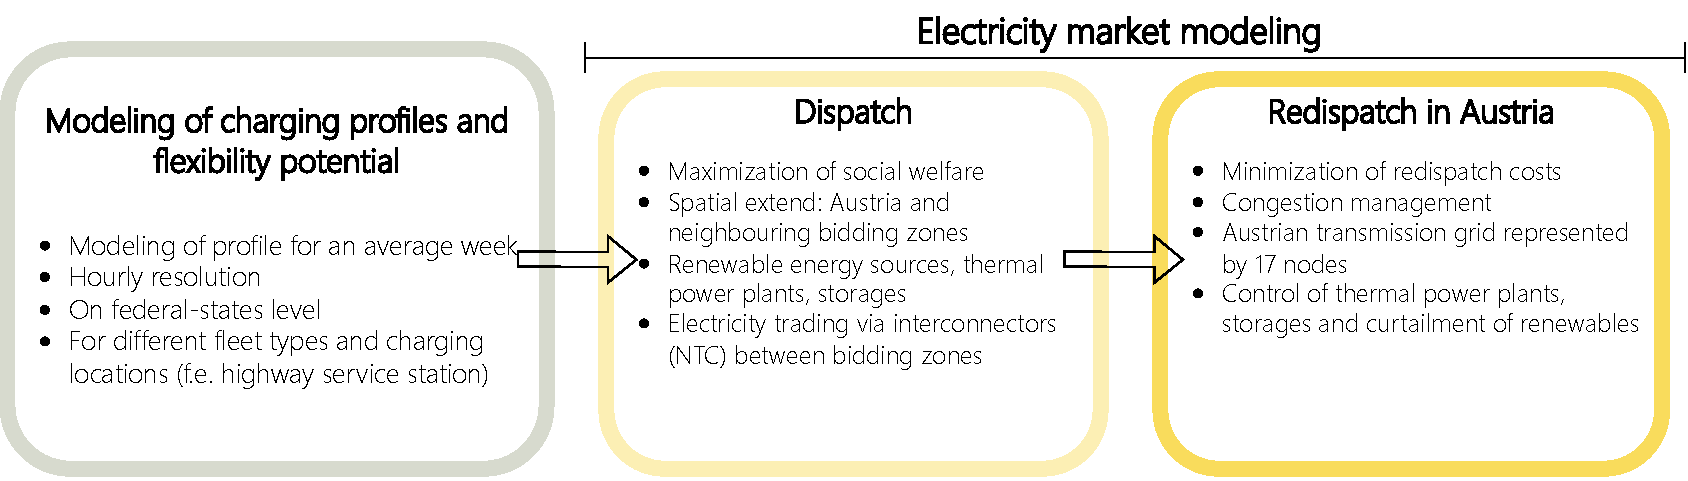
\includegraphics[width=0.9\textwidth]{graphics/overview_model_3_steps.drawio.pdf}
            \caption{Overview of the steps of the methodology}
            \label{fig:model_overview}
        \end{figure}

        \begin{figure}[h]
            \centering
            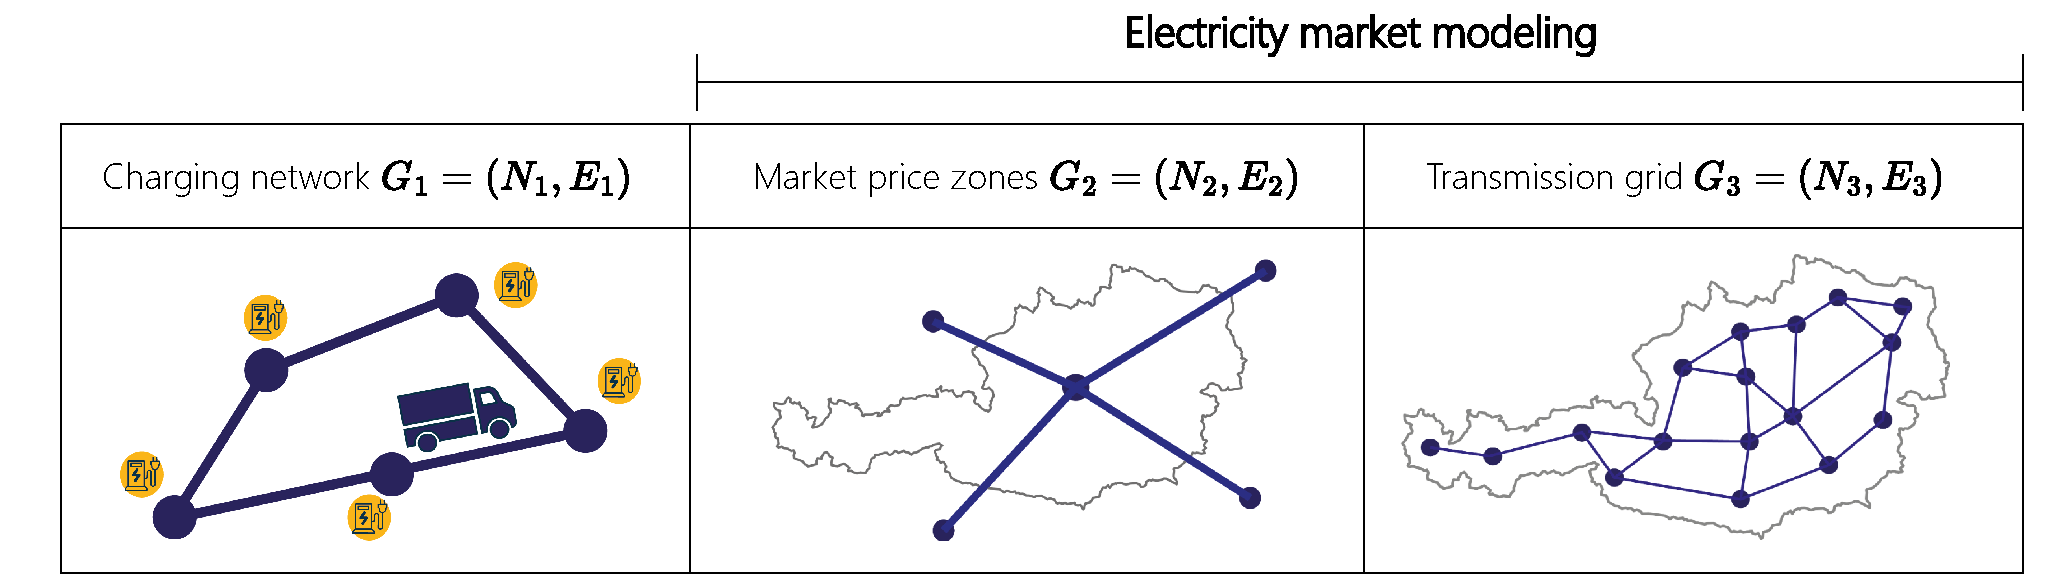
\includegraphics[width=1\textwidth]{graphics/overview_graphs.drawio.pdf}
            \caption{The three layers of geographic information used throughout the methodology.}
            \label{fig:model_graphs}
        \end{figure}


    \subsection{Mathematical framework}
        \subsubsection{Definition of the flexibility potential}
        Figure \ref{fig:flexibility_potential_detail} describes the definition of the flexibility potential in the charging of vehicles graphically as a function of time and the state of charge: A vehicle is connected to a charging station for a defined period during which a certain amount of electricity must be charged. In the present example, the battery needs to be recharged until its maximum capacity, $\mathrm{SOC}^{\mathrm{BEV max}}$. An initial charging profile is given based on an assumption of the charging strategy of the vehicle. In the illustrated case, this charging strategy is charging at the lowest possible continuous power level ($\mathrm{CAP}^{\mathrm{BEV const}}$), distributing the charged energy evenly during the plug-in period (indicated with the dark red line). A maximum possible charging power, $\mathrm{CAP}^{\mathrm{BEV max}}$, \added{defines the inclination of the green lines and, therefore, the}
        time span of the fastest possible charging process and the latest possible point in time at which the charging process must start in order to fully recharge\deleted{( green lines)}. The orange line illustrates an example of a load curve with a variable power level, with the power level at the beginning and at the end being significantly higher than during the mid-part of the plug-in period. The area bounded by the green oblique lines indicates the extent of possible charging curves to reach $\mathrm{SOC}^{\mathrm{BEV max}}$ during the plug-in time period, which translates to the flexibility potential of the charging process. \added{For example, in fast-charging processes where the charging happens at $\mathrm{CAP}^{\mathrm{BEV max}}$ and the plug-in period is closer to the point of "fastest achievable charging completion", flexibility is more limited.}

            \begin{figure}[h]
                \centering
                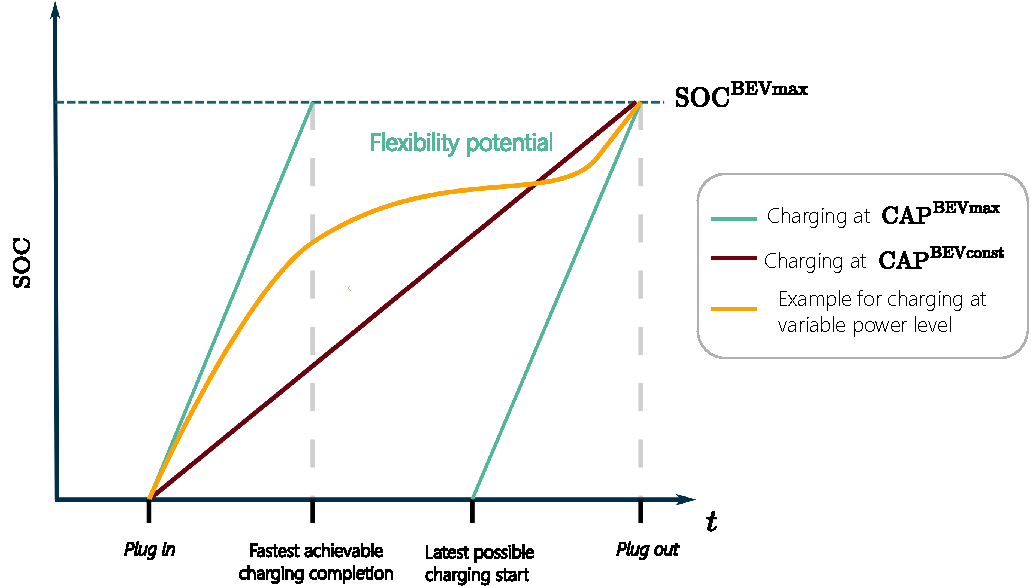
\includegraphics[width=0.8\textwidth]{graphics/flexibility_potential.drawio.pdf}
                \caption{Graphic illustration of the flexibility of a charging process}
                \label{fig:flexibility_potential_detail}
            \end{figure}

        \subsubsection{Modeling of the charging profiles} \label{sec:modeling_charging}
            The spatial and temporal distribution of charging demand is determined independently. The charging profiles in this analysis are generated and scaled for each fleet type in a different way due to varying operation patterns. We differentiate between two types of operation patterns: local and interregional transport, assigning each fleet to the groups $\mathcal{F}^{\mathrm{local}}$ and $\mathcal{F}^{\mathrm{inter}}$.

            \paragraph{Local transport}
                For the case of local transport, the charging demand of a vehicle is assigned to exclusively one node in $\mathcal{G}_1$. We aggregate all vehicles of a specific type to a fleet $f \in \mathcal{F}^{\mathrm{local}}$ and the energy demand for node $n$ is estimated as follows:
                \begin{align}
                    D^{\mathrm{BEV}}_{f,n} = \overline{D^{\mathrm{spec,BEV}}_{f}} \cdot dist_{f}  \cdot k_{f,n} \quad \forall f \in \mathcal{F}^{\mathrm{local}}, n \in \mathcal{N}_1 \\
                    \sum_{l \in \mathcal{L}^f} D^{\mathrm{BEV}}_{f,n,l} = D^{\mathrm{BEV}}_{f,n}  \quad \forall f \in \mathcal{F}^{\mathrm{local}}, n \in \mathcal{N}_1
                \end{align}
                The charging demand during the observed time period is deducted from the distance $dist_f$ that is driven by a vehicle of fleet $f$, its energy consumption $\overline{D^{spec,\mathrm{BEV}}_{f}}$ and the amount of the vehicles of fleet type $f$ operating at node $n$ $k_{f,n}$ is. The charging demand is assigned to different charging locations $\mathcal{L}^f$ that are available to the fleet. These are, for example, depots at node $n$. Each charging location type is characterized by an installed maximum charging power $\mathrm{CAP}^{\mathrm{BEV max}}_{f, n, l}$. The particular distribution of the charging demand to the charging location is conducted based on the assumed charging strategy for this fleet. 
            
                \paragraph{Interregional transport}
                For interregional transport, vehicles are assumed to travel between regions and charge at more than one node. In this case, a set of routes is given for the fleet $R^f = \{R_1, R_2, \dots R_I\}, i=1,2, \dots I$. The routes are all allocated in graph $\mathcal{G}_1$. The charging demand is determined and assigned to nodes $n \in \mathcal{N}_1$ for each route separately and later aggregated at each node for all considered types of charging locations. Each route $R_i$ is traveled by a part of the fleet,  $f_i \in \mathcal{F}^{\mathrm{inter}}$. Charging locations are either allocated along the route $\mathcal{L}^{\mathrm{enroute}}_f$ or at origin and destination nodes $\mathcal{L}^{f, \mathrm{OD}}$. In accordance with this, the nodes contained in a route are categorized into two sets: $\mathcal{N}_{i}^{\mathrm{enroute}}$ and  $\mathcal{N}_{i}^{\mathrm{OD}}$. 
                \begin{flalign}
                   &\hfill D^{\mathrm{BEV}}_{f_i} = dist_i \cdot \overline{D^\mathrm{spec,BEV}}_{f} \cdot k_i \\
                   &\hfill = \sum_{n \in \mathcal{N}_i^{\mathrm{enroute}}} \sum_{l \in \mathcal{L}^{\mathrm{enroute}}_f}  D^{\mathrm{BEV}}_{f_i, n, l}  + \sum_{n \in \mathcal{N}_i^{\mathrm{OD}}} \sum_{l \in \mathcal{L}^{\mathrm{OD}}_f}  D^{\mathrm{BEV}}_{f_i, n, l} \nonumber \\  &\hfill\forall i = 1, 2, \dots I, f \in \mathcal{F}^{\mathrm{inter}} \nonumber
                \end{flalign}
        
            $k_i$ defines the number of vehicles traveling on the route $R_i$ in the observed period. The charging demand for this route is distributed between the locations positioned along the route and at the origin or destination nodes. The particular assignment of the magnitude of charging demand to the nodes, $ D^{BEV}_{f_i, n, l}$ depends further on the assumed charging strategy.
        
        \paragraph{Nodal aggregation and temporal distribution}
            We aggregate the charging demand for each fleet type and the respective locations on node-level: 
            
            \begin{flalign}
                D^{\mathrm{BEV}}_{f,n,l} =
                  \begin{cases}
                    D^{\mathrm{BEV}}_{f,n,l}       & \quad \text{if } f \in \mathcal{F}^{\mathrm{local}}\\
                    \sum_{i} D^{\mathrm{BEV}}_{f_i, n, l} & \quad \text{if } f \in \mathcal{F}^{\mathrm{inter}}
                  \end{cases}
            \end{flalign}
                
        
            The plug-in periods are during periods of operational downtime of the vehicles, during operation times only when needed. Independently of obtaining the absolute magnitude for each fleet, the charging demand is assigned to timestep $t \in \mathcal{T}$:
            \begin{align}
                D^{\mathrm{BEV}}_{f,n,l, t} = g(D^{\mathrm{BEV}}_{f,n,l}, t)
            \end{align}
            $g(\cdot)$ indicates here the function assigning the amount of charging load to each time, resulting in a charging demand defined for each time step, $D^{BEV}_{f,n,l,t}$.

    \subsubsection{Electricity market modeling}
        The European electricity market model \textit{EDisOn} \cite{LOSCHAN2023108802,LOSCHAN2024109992} is a linear programming unit commitment model that encompasses the European electricity market and national hydrogen markets. The objective is the minimization of the overall dispatch costs to meet the electricity demand plus hydrogen production revenues of the market area, being the dual problem to social welfare maximization. The model calculates the minimal dispatch cost of all thermal power plants, the curtailment of \ac{RESE}, and storage use to meet the electricity demand while maximizing hydrogen production revenues. The demand for electricity is made up of exogenous inelastic demand and flexible demand. This flexible demand includes the flexibility of hydrogen production and the demand for electrified commercial transport. The generation of renewable energy source technologies, namely photovoltaic, run-of-the-river hydroelectricity, and wind, are not dispatchable, and their generation profiles are exogenously defined. A reduced set of nodes $n \in \mathcal{N}_2$ with one node per bidding zone is used to determine the optimal dispatch from an economic perspective (Figure \ref{fig:model_graphs}). These nodes are connected with a reduced grid model constrained by the interconnectors. Hence, congestion of transmission lines within a country can occur. The dispatch optimization is performed as a rolling horizon optimization with 26 optimization steps including 336 hours each.

        After the dispatch optimization, a more detailed model for Austria, with 17 nodes ($n \in \mathcal{N}_3$), is used to determine congestion and calculate the cost-optimal redispatch to overcome congestion \added{in the transmission grid}. Thus, the differences between the market-based optimum and the actual physical power flows are analyzed.
        The previously dispatched power plants are then assigned to the respective nodes using their existing generation schedules. Power flows are calculated using a direct current power flow approximation. The decision variables of the dispatch remain unchanged and are applied as parameters in the redispatch optimization. The redispatch needs are balanced cost-minimal by new decision variables that adjust the generation of thermal power plants, storages, additional curtailment of \ac{RESE} and the use the commercial \ac{BEV} fleet demand-side flexibility. The redispatch optimization is performed for blocks of 24 hours. 

        In the following mathematical description, the decision variables in the current study are always written in lower case, and endogenously defined constants are written using upper case letters. Only the equations that are most relevant to the present work are stated here. We explain the most relevant parameters and variables here, while a detailed overview on all is given in the \ref{sec:Appendix_nomenclature}.

        \paragraph{Dispatch} 
            The objective function (Equation \ref{equ:objective_function}) minimizes the overall costs for electricity generation $q$. These costs encompass costs of thermal power plant ($\mathrm{TH}$) generation, including the short-run marginal costs of generation of thermal power plants ($\mathrm{SRMC}$), and their start-up costs ($C^{\mathrm{start}}$), as well as operation and maintenance for pumped hydro-power storage units ($ps \in \mathcal{PS}, q^{\mathrm{tu}} \cdot C^{\mathrm{ps}}$). Further, for renewable energy sources for electricity (RESE), specific operation and maintenance costs are considered, which are multiplied from the endogenously assumed generation ($Q^{\mathrm{RESE}}$) and the curtailed RESE generation ($\mathrm{spill}^{\mathrm{RESE}}$). We introduce a fee ($\mathrm{VoLL}$) for not supplied energy ($\mathrm{nse}$), and cost and revenues from producing hydrogen ($q^{\mathrm{H_2}}_{\mathrm{el},ey}$) by electrolyzers, $ey \in \mathcal{EY}$, and covering hydrogen demand ($d^{\mathrm{H_2}}_{\mathrm{el}}$) of fuel cells, $fc \in \mathcal{FC}$, considering the exogenous hydrogen market price $P^\mathrm{bid}_{\mathrm{H_2}}$.

            \begin{flalign} 
            \label{equ:objective_function}
            &\underset{q, \mathrm{str}, q^\mathrm{tu}, \mathrm{spill}^{\mathrm{RESE}}, \mathrm{nse}, q^{\mathrm{H_2}}_\mathrm{el}, d^{\mathrm{H_2}}_{\mathrm{el}}}{\mathrm{minimize}} 
            \\ \nonumber
            & \sum_{t \in \mathcal{T}} \sum_{th \in \mathcal{TH}} \left( q_{t,th} \cdot \mathrm{SRMC}_{th} + \mathrm{str}_{t,\mathrm{th}} \cdot C^{\mathrm{start}}_{th} \right)  
            + \sum_{t \in \mathcal{T}} \sum_{ps \in \mathcal{PS}} q^\mathrm{\mathrm{tu}}_{t,ps} \cdot C^{\mathrm{ps}}_{ps} 
            \\ \nonumber
            + &\sum_{t \in \mathcal{T}} \sum_{r \in \mathcal{RESE}}
            \left( Q^{\mathrm{RESE}}_{t} - \mathrm{spill}^{\mathrm{RESE}}_{t,r} \right) \cdot C^{\mathrm{RESE}}
            + \sum_{t \in \mathcal{T}} \sum_{n \in \mathcal{N}_2} \mathrm{nse}_{t,n} \cdot \mathrm{VoLL} \\ \nonumber
            - & \sum_{t \in \mathcal{T}} \sum_{ey \in \mathcal{EY}} P^\mathrm{bid}_{\mathrm{H_2}} \cdot q^{\mathrm{H_2}}_{\mathrm{el}, t,ey} + 
            \sum_{t \in \mathcal{T}} \sum_{fc \in \mathcal{FC}} P^\mathrm{bid}_{\mathrm{H_2}} \cdot d^{\mathrm{H_2}}_{\mathrm{el}, t,fc} \\
            \nonumber
            \end{flalign}

            
            This optimization problem is solved subject to several constraints. The demand that must be met in every node for each timestamp (Equation \ref{equ:dispatch_kirchhoff}) employs the exogenous electricity demand ($D_{n}$) and the flexible, temporal shift-able electrified commercial \ac{BEV} fleet demand ($d^\mathrm{BEV}_{n}$). The dual variable of this constraint ($p^{CP}$) provides the day-ahead price per bidding zone as an hourly profile. This price is used in the redispatch step to evaluate the cost of redispatch measures.
            \begin{flalign} \label{equ:dispatch_kirchhoff} 
            &D_{t,n} + d^\mathrm{up}_{t,n} - d^\mathrm{down}_{t,n} + d^\mathrm{BEV}_{t,n} + \displaystyle\sum\limits_{ey \in \mathcal{EY}_{n}} d^\mathrm{el}_{\mathrm{H_2},t,e} = \\ \nonumber
            & \displaystyle\sum\limits_{th \in \mathcal{TH}_{n}} q_{t,\mathrm{th}} + \displaystyle\sum\limits_{fc \in \mathcal{FC}_{n}} q^\mathrm{el}_{\mathrm{H_2},t,fc} + 
            \displaystyle\sum\limits_{ps\in \mathcal{PS}_{n}} (q^{tu}_{t,{ps}} - q^\mathrm{pu}_{t,{ps}}) 
            + \displaystyle\sum\limits_{{st} \in \mathcal{ST}_{n}} (q^\mathrm{out}_{t,{st}} - q^\mathrm{in}_{t,{st}}) \\ \nonumber
            &+ Q^\mathrm{RESE}_{t,n} - \mathrm{spill}^\mathrm{RESE}_{t,n} - \mathrm{exch}_{t,n} + \mathrm{nse}_{t,n} : p^\mathrm{CP}_{t,n}\\ \nonumber
            &\forall t \in \mathcal{T}, \forall n \in\mathcal{N}_2 
            \end{flalign}

            The flexibility provided by the electrified commercial fleet is implemented as the summation of fleet- and charging-location-specific charging demands ($D^\mathrm{BEV}$) and their positive ($d^\mathrm{BEV +}$) and negative demand regulation ($d^\mathrm{BEV -}$). This represents an aggregated demand per node ($d^\mathrm{BEV}$) as described in Equation \ref{equ:EV_aggregation}.
            \begin{flalign} 
                &d^\mathrm{BEV}_{t,n} = \displaystyle\sum\limits_{f \in \mathcal{F}}\sum\limits_{l \in \mathcal{L}^f} D^\mathrm{BEV}_{f, n, l, t} + d^\mathrm{BEV +}_{f, n, l, t} - d^\mathrm{EV -}_{f, n, l, t} \label{equ:EV_aggregation} \\ \nonumber
                &\forall t \in \mathcal{T}, \forall n \in \mathcal{N}_2
            \end{flalign}
            A demand increase (Equation \ref{equ:EV_curtailment_up}) and decrease (Equation \ref{equ:EV_curtailment_down}) is only possible when the initial charging demand is larger than zero, thereby implying that the \ac{BEV}s are connected to a charging station. The upper power limit ($\mathrm{CAP}^\mathrm{BEV max}$) must not be exceeded and the charging power must not be lower than the minimum power ($\mathrm{CAP}^\mathrm{BEV min}$).
            \begin{flalign} 
                &d^\mathrm{BEV +}_{f,n, l,t} = 0 ;\quad \forall D^\mathrm{BEV}_{f,n, l,t} \leq 0 
                \label{equ:EV_curtailment_up}\\ \nonumber
                &0 \leq d^\mathrm{BEV +}_{f,n, l,t} \leq \mathrm{CAP}^\mathrm{BEV max}_{f,n, l,t} - D^\mathrm{BEV}_{f,n, l,t} ;\quad \forall D^\mathrm{BEV}_{f, n, l, t} > 0 \\
                &d^\mathrm{BEV -}_{f,n,l,t} = 0 ;\quad \forall D^\mathrm{BEV}_{f,n, l,t} \leq 0
                \label{equ:EV_curtailment_down} \\ \nonumber
                &0 \leq d^\mathrm{BEV -}_{f,n, l,t} \leq D^\mathrm{BEV}_{f,n,l,t} - \mathrm{CAP}^\mathrm{BEV min}_{f, l} ;\quad \forall D^\mathrm{BEV}_{f,n,l,t} > 0 \\ \nonumber
                &\forall f \in \mathcal{F}, n \in \mathcal{N}_2, l \in \mathcal{L}, t \in \mathcal{T} 
            \end{flalign}
            \added{Equation \ref{equ:EV_charging_guarantee} ensures that the electricity demand of each charging demand is always compensated whilst the vehicle is plugged in. During this time frame, a demand regulation is possible. Because there is never more than one plug-in timeframe per 24 hours, it is possible to implement the constraint as the sum over these 24 hours.}
            \begin{flalign}
                 &\displaystyle\sum\limits_{t=j\cdot24+13}^{t=j\cdot24+36} d^\mathrm{BEV +}_{f,l,t} - d^\mathrm{BEV -}_{f,l,t} = 0 \label{equ:EV_charging_guarantee} \\ \nonumber
                 &\forall f \in \mathcal{F}, l \in \mathcal{L}, \forall j \in \left\{0,1,...,\frac{T}{24}-2 \right\}
             \end{flalign}
            \paragraph{Redispatch}
            The redispatch optimization modificates the generation schedules determined in the dispatch to balance redispatch needs. This is associated with costs that are minimized (Equation  \ref{equ:redispatch_objective_function}). These costs arise due to the increase in thermal power plant generation and the use of hydro and battery storage.
        \begin{flalign}
            &\underset{q^\mathrm{+ Redis},q^\mathrm{- Redis},q^{tu Redis},q^{pu Redis},q^{out Redis},q^{in Redis}}{\mathrm{minimize}}
            \label{equ:redispatch_objective_function} \\ \nonumber
            &\sum_{t \in \mathcal{T}} \sum_{{th} \in \mathcal{TH}_\mathrm{AT}} \left( q^\mathrm{+ Redis}_{t,{th}}  \cdot C^\mathrm{th Redis}_{t,{th}} 
                - q^\mathrm{- Redis}_{t,{th}}  \cdot \mathrm{SRMC}_{th} \right)\\  \nonumber
            &+ \sum_{t \in \mathcal{T}} \sum_{{ps} \in \mathcal{PS}_\mathrm{AT}} \left(q^{\mathrm{tu Redis}}_{t,ps} + q^{\mathrm{pu Redis}}_{t,ps}\right)
            + \sum_{t \in \mathcal{T}} \sum_{{st} \in \mathcal{ST}_\mathrm{AT}} \left(q^{\mathrm{out Redis}}_{t,st} + q^{\mathrm{in Redis}}_{t,st}\right)
        \end{flalign}
         The costs of a thermal generation increase ($C^\mathrm{th Redis}$) as redispatch measure is the same as the day-ahead market price or the SRMC if these are higher (Equation \ref{equ:redis_thermal_costs}). Thermal power plant generation decrease leads to refund proportional to the respective short-run marginal costs. Storage use leads to costs proportional to the day-ahead market price. 
        \begin{flalign} 
            &C^\mathrm{th Redis}_{t,{th}} = \mathrm{max}\left(P^\mathrm{CP}_{t,n_{th}}, \mathrm{SRMC}_{th}\right)
            \label{equ:redis_thermal_costs} 
        \end{flalign} 
        The demand compensation constraint (Equation \ref{equ:dispatch_kirchhoff}) is expanded by the additional redispatch decision variables (Equation \ref{equ:redispatch_kirchhoff}). The generation schedules are taken over from the dispatch; thus, the redispatch regulation must be used if necessary. This constraint is only used within Austria because the redispatch evaluation is conducted in this country. In contrast to the market-based dispatch, all transmission lines and nodes in Austria are considered ($\mathcal{N}_3$). Because redispatch measures within Austria will marginally change the power flow over the whole market area and all transmission lines all other bidding zones serve as slack.
        \begin{flalign} \label{equ:redispatch_kirchhoff}
        &D_{t,n} + D^\mathrm{up}_{t,n} - D^\mathrm{down}_{t,n} + d^\mathrm{BEV}_{t,n} + \displaystyle\sum\limits_{e \in \mathcal{EY}_{n}} D^\mathrm{el}_{\mathrm{H_2},t,e} = \\ \nonumber
        &\displaystyle\sum\limits_{{th} \in \mathcal{TH}_{n}} Q_{t,{th}} + q^\mathrm{+ Redis}_{t,{th}} - q^\mathrm{- Redis}_{t,{th}} + \displaystyle\sum\limits_{{fc} \in \mathcal{FC}_{n}} Q^\mathrm{el}_{\mathrm{H_2}, t,{fc}} \\ \nonumber
        &+ \displaystyle\sum\limits_{{ps} \in \mathcal{PS}_{n}} (Q^\mathrm{tu}_{t,{ps}} + q^{tu Redis}_{t,ps} - Q^\mathrm{pu}_{t,{ps}} - q^{pu Redis}_{t,ps}) \\ \nonumber
        &+ \displaystyle\sum\limits_{{st} \in \mathcal{ST}_{n}} (Q^\mathrm{out}_{t,{st}} + q^{out Redis} - Q^\mathrm{in}_{t,{st}} - q^{in Redis}_{t,st}) \\ \nonumber 
        &+ Q^\mathrm{RESE}_{t,n} - \mathrm{Spill}^\mathrm{RESE}_{t,n} - \mathrm{spill}^\mathrm{RESE}_{\mathrm{Redis},t,n} - \mathrm{exch}_{t,n} + \mathrm{NSE}_{t,n} \\ \nonumber
        &\forall t \in \mathcal{T}, \forall n \in \mathcal{N}_3
        \end{flalign}
                
        \added{Further details on the dispatch and redispatch optimization model, such as the constraints for flow and line capacity limits, can be in the paper by \citet{LOSCHAN2023108802}.}
        \subsection{Data and materials} \label{sec:data}
                    The methodological framework is applied to Austria in 2040. In the following, we describe the parametrization of the analysis.
        \subsubsection{Future charging demand of Austrian electrified commercial fleet}
            The representation of the commercial fleet is focused on three fleet types: \aclp{LDT}, \aclp{HDT}, and buses. These are chosen based on their substantial fleet size and transport activity. Their electrification is therefore expected to play a significant role in the electricity system. Based on the mobility patterns of the different fleet types and expected charging strategies, future charging profiles are generated together with plug-in times and installed charging power. The charging profiles are generated for an average week in 2040, i.e. representing seven days in hourly resolution. The theoretical framework presented in Section \ref{sec:modeling_charging} is the starting point for the estimation of future charging profiles. In the geographic aggregation of charging profiles, Austria is represented by nine nodes ($|\mathcal{N}_1|=9$) mirroring the nine federal states of Austria.

            \paragraph{Light-duty trucks}
            % https://www.oesterreich.gv.at/themen/mobilitaet/kfz/Seite.061800.html#KlasseN
            The \ac{LDT} fleet classified as vehicles that have a maximum total weight of 3.5 tons \cite{usp_nutzfahrzeuge}. The Austrian vehicle fleet of this type amounted to a size of around 510,000 vehicles by the end of 2023 and is expected to be 535,000 by 2040 in decarbonization scenarios by \citet{umweltbundesamt_rep0808}. According to \cite{SCORRANO2021101022}, the \added{average} daily range of a light-duty vehicle operated in Germany is 70km on average. We adopted this value for Austria. Further assumptions for the vehicle are summarized in Table \ref{tab:parameters_ldv}. Based on this, we assume the routes of vehicles of this fleet type to only within one Federal State and, therefore, the charging profile of the \ac{LDT} fleet is modeled based on the operational pattern of \textit{local transport}. 

            The core assumptions for the modeling of a charging profile of light-duty vehicles are the following:
            \begin{itemize}
                \item \textbf{Charging strategy:} Vehicles are charged during nighttime and weekends. Recharging is done at depots. During weekends, the vehicles have a substantially higher flexibility in the recharging processes. The charging process is performed at the lowest possible power level and is evenly distributed during the plug-in period. Departure times are evenly distributed between 7 am and 9 am, and arrival times are between 16 pm and 18 pm.
                \item \textbf{Geographic scaling:} The expected amount of \ac{LDT} is distributed proportionally to the population size.
                \item \textbf{Sizing of charging infrastructure:} The aggregated charging infrastructure for all depots within a federal state region is sized based on assuming that the charging power of 11kW and charging the vehicle every sixth night is sufficient.
            \end{itemize} 

            \paragraph*{Heavy-duty truck}
            The \ac{HDT} has a total weight greater than 3.5 tons. Technical assumptions for this fleet are summarized in Table \ref{tab:parameters_hdv}. Origin-destination flow data on the European level is used here to capture charging demand from national as well as transit transport. The ETISplus dataset provides estimations of the annual tons transported by trucks in the year 2030 \cite{speth2021synthetic}. We apply the charging profile generation for \textit{interregional transport} here under the following considerations:
            
            \begin{itemize}
                \item \textbf{Charging strategy:} For this we consider that the European regulation dictates a maximum driving shift of 4.5 hours. \ac{HDT}s are charged at depots and highway service areas \cite{ec_driving_time_2023}. Further, in Austria, a regulation prohibits driving between 10 pm and 5 am for multiple transport segments \cite{usp_lkw_fahrverbote}. During Saturdays and Sundays, the operation of heavy-duty transport is also restricted. For trips that take longer than 4.5 hours, the 45-minute break takes place at a highway service area, and during this time, the \ac{HDT} is connected to a megawatt charging station and is fully charging. The remaining energy demand is covered at the origin and the destination depots during nighttime. For trips shorter than 4.5 hours, charging is fully compensated at depots. Recharging happens also at depots during the day if the driving range is not sufficient to be covered with one charged battery. During trips that take multiple days, charging demand is also compensated at service areas during nighttime. 

                \item \textbf{Sizing of charging infrastructure:} Charging in depots is assumed to be conducted at 100kW of peak power and megawatt charging is available at charging stations. As a reference point for the sizing of charging infrastructure, the goals for the installment of 5MW of grid connection at each charging station until 2035/2040 along the Austrian highway network by the highway infrastructure operator ASFINAG \cite{ioebenergiespeicher}\footnote{The exact number of 5MW was stated by a representative of ASFINAG in the course of a stakeholder interview.}. This is assumed to be available for the electrification rate of a heavy-duty fleet of 30\%. A relative factor to the charging demand is deducted for each region based on the amount of existing service areas and applied to all charging location demands within the respective region. 

                \item \textbf{Flexibility in the fast-charging along highway service areas:} Due to the short time frame of the break of 45 minutes and the used temporal resolution of the modeling being one hour, there is no flexibility given for highway charging processes. It may be foreseeable that the operational times and the timing of the break and, therefore, the charging process would be adapted to charge for lower expenses in the future. Therefore, to introduce some flexibility here, we created three distinct plug-in time frames of two hours each, which are allocated around noon. 
        
            \end{itemize}
            
        \paragraph*{Busses}
        For the bus fleet, we consider the application case for public transport in both cities and rural regions. Similar to the modeling of light-duty vehicles, the routes of buses do not go through multiple regions. Table \ref{tab:parameters_bus} comprises technical assumptions for an average bus in public transport.

            The charging profiles for busses are estimated based on the following:
            \begin{itemize}
                \item \textbf{Charging strategy:} Most charging demand is covered during night time at the bus depot. If required, busses enter the depot for fast charging during daytime. The operation is assumed to be similar during each day of the week.
                % \item \textbf{Charging locations:} All busses are charged in a bus depot.
                % \item \textbf{Temporal distribution:} All busses are assumed to operate similarly each day of the week. They are preferably charged at night, outside of the main operating hours. City buses have a higher daily consumption than applied in rural areas, which exceeds the size of the battery pack. Therefore, city buses compensate for this through fast charging during the day in the depot. 
                \item \textbf{Geographic scaling:} City busses are considered for Austrian cities that surpass the population size of 100,000. For each city, the size of the bus fleet is scaled using the population size. The bus fleet in rural areas is sized using the total area of the rural region within a federal state.  
                \item \textbf{Sizing of charging infrastructure:} During night time, each bus is connected to a 100kW charging station. The power connection of the depot is limited to two-thirds of the summed peak power of the charging stations which is sufficient to cover the charging demand during down times at night and is in line with the peak power achieved with coordinated and, therefore, cost-efficient charging \cite{Borlaug2021}. 
            \end{itemize}

        \begin{table}[]
        \centering
        \caption{Parameter settings for modeling the charging demand of light-duty vehicles}
        \label{tab:parameters_ldv}
        \begin{tabular}{@{}lrl@{}}
        \toprule
        \textbf{Parameter}                       & \multicolumn{1}{l}{\textbf{Value}} & \textbf{Reference} \\ \midrule
        Fleet size (Austria 2040)                & 535,000                            &   \cite{umweltbundesamt_rep0808}                 \\
        Battery capacity                         & 145 kWh                            &      \cite{irena2019smart_charging}              \\
        Specific energy consumption              & 27 kWh/100km                       &     \cite{umweltbundesamt_rep0808}              \\
        Daily range                              & 70 km/day                          &  \cite{SCORRANO2021101022}                   \\
        Charging power at charging station depot & 11 kW                              &        \cite{SCORRANO2021101022}             \\ \bottomrule
        \end{tabular}%
        
        \end{table}


        % Please add the following required packages to your document preamble:

        \begin{table}[]
        \centering
        \caption{Parameter settings for modeling of charging profile of heavy-duty vehicles}
        \label{tab:parameters_hdv}
        \begin{tabular}{@{}lrl@{}}
        \toprule
        \textbf{Parameter} &
          \multicolumn{1}{l}{\textbf{Value}} &
          \textbf{Reference} \\ \midrule
        Battery capacity &
          350 kWh & \cite{teoh2022}
           \\
        Specific energy consumption &
          1.3 kWh/km &
          \cite{umweltbundesamt2024}  \\
        Average load &
          10.63 tons &
           \cite{umweltbundesamt2024} \\
        Average driving speed &
          50 km/h & \cite{9543135} 
           \\
        \begin{tabular}[c]{@{}l@{}}Peak charging power at highway/depot charging station \\ (fast charging during daytime)\end{tabular} &
          1000 kW &
           \\
        \begin{tabular}[c]{@{}l@{}}Peak charging power at highway/depot charging station\\ (slow charging during nighttime)\end{tabular} &
          100 kW &
           \\ \bottomrule
        \end{tabular}%
        
        \end{table}

        % Please add the following required packages to your document preamble:
        %usepackage{booktabs}
        % usepackage{graphicx}
        \begin{table}[]
        \centering
        \caption{Parameter settings for the modeling of charging profile by busses in the application in the city and rural areas}
        \label{tab:parameters_bus}
        \begin{tabular}{@{}lll@{}}
        \toprule
        \textbf{Parameter}          & \textbf{Value} & \textbf{Reference} \\ \midrule
        Fleet size (Austria 2040)   & 12,900         &            \begin{tabular}[c]{@{}l@{}}extrapolated \\ based on \cite{wienerlinien2024}, \cite{vmobil2023}\end{tabular}          \\
        Battery capacity & 350 kWh     &              \cite{ag2022flexibility}    \\
        Specific energy consumption & 1.3 kWh/km     &               \cite{umweltbundesamt2024}    \\
        Daily range - city        & 236 km         &     \cite{wienerlinien2024}              \\
        Daily range - rural       & 138 km         &     \cite{vmobil2023}               \\
        \begin{tabular}[c]{@{}l@{}}Peak charging power at depot charging station\\ (fast charging during daytime)\end{tabular}   & 1000 kW &  \\
        \begin{tabular}[c]{@{}l@{}}Peak charging power at depot charging station\\ (slow charging during nighttime)\end{tabular} & 100 kW  &  \\ \bottomrule
        \end{tabular}%
        
        \end{table}
        % Please add the following required packages to your document preamble:
        % \usepackage{booktabs}
        % \usepackage{graphicx}
        \begin{table}[]
        \centering
        \caption{Electrification scenarios considered in the analysis}
        \label{tab:parameters_scenario}
        \begin{tabular}{@{}lrrr@{}}
        \toprule
                        & \multicolumn{3}{l}{Share of electrification in fleet} \\ \cmidrule(l){2-4} 
        Scenario & \multicolumn{1}{l}{Light-duty vehicles} & \multicolumn{1}{l}{Heavy-duty vehicles} & \multicolumn{1}{l}{Busses} \\
        \textit{LOW}    & 100\%            & 30\%             & 100\%           \\
        \textit{MEDIUM} & 100\%            & 50\%             & 100\%           \\
        \textit{HIGH}   & 100\%            & 100\%            & 100\%           \\ \bottomrule
        \end{tabular}%
        
        \end{table}
        \subsubsection{Electricity market 2040} 
        All 13 countries (Austria, Germany, Netherlands, Belgium, Luxembourg, Czech Republic, Slovenia, Switzerland, Poland, Slovakia, Hungary, Italy, and France) within the optimized area are expected to fulfill the European national energy and climate plans \cite{NECP2022} by 2030 and continue to compensate for the rising electricity demand by expanding generation capacities in 2040. According to Austria's national energy and climate plans, \ac{RESE} compensates for 100\% of the yearly electricity demand. The used \textit{National Trends} dataset, provided by the European Network of Transmission System Operators for Electricity is based on the fulfillment of these plans \cite{TYNDP2022}. It includes a power plant fleet with \ac{RESE}, fossil fuel-fired power plants (coal, oil, lignite, and combined-cycle gas turbines, and other types of thermal power plants that do not emit CO\textsubscript{2} (nuclear, biogas, biomass, and fuel cells).
        
        \subsubsection{Scenarios and case studies}
            In the application to the Austrian electricity system in 2040, we explore two different dimensions: On the one side, the variation in the share of electrification of the commercial fleet in 2040, and, on the other side, the role of the commercial \ac{BEV} fleet in the electricity market. Table \ref{tab:parameters_scenario} displays the shares of electrification for the three considered electrification scenarios, \textit{LOW}, \textit{MEDIUM}, and \textit{HIGH}. The three case studies for market participation describe:
    
            \begin{itemize}
                \item \textbf{Baseline:} The charging demand of the commercial \ac{BEV} fleet is inflexible.
                \item \textbf{Dispatch:} The flexibility of the charging of the commercial \ac{BEV} fleet is optimized in the dispatch.
                \item \textbf{Redispatch:} The flexibility of the commercial \ac{BEV} fleet charging is utilized in redispatch measures.  
            \end{itemize}


\section{Results}

    The structure of this section follows the sequence of the analyzed case studies for Austria in 2040: First, the modeled charging demand and profiles are presented (case study \textit{Baseline}). Second, we describe how the charging load profiles are shifted as a result of the contribution of the charging flexibility to the day-ahead market (case study \textit{Dispatch}). Further, we look into the participation of the commercial \ac{BEV} fleet as redispatch measures to overcome congestion (case study \textit{Redispatch}). Here, we particularly showcase the relevancy of the consideration of the spatial variation of the charging demand.
    
    % First, the demand 
    % We start here with an overview of the results of charging demand and charging profiles. After this, the charging load as a result of market participation in the dispatch is presented, giving an insight into how the assumed charging profile (\textit{Baseline} case) is changed when coordinated with the electricity pricing. We further look into the potential of using smart charging in redispatch measures and go deeper into spatial differences in the alteration of the \textit{Baseline} charging profiles to showcase the relevancy of the consideration of spatial variation of charging demand in this analysis. 


    % \begin{itemize}
    %     \item Results of the modelling of charging profiles --- cumulated and spatial distribution
    %     \begin{itemize}
    %         \item table of cumulative annual demand -- check
    %         \item image for peaks at highway charging areas -- check
    %         \item image for regional peaks, implicating national distribution and regions were more needs to be developed -- check
    %     \end{itemize}
    %     \item Temporal distribution of the load and the temporal shift in dispatch and redispatch model + 
    %     \begin{itemize}
    %         \item Temporal distribution + dispatch profile + electricity prices -- check 
    %         \item Temporal distribution + redispatch profile + electricity prices -- check ( this does not need electricity prices in it! - remove) 
    %         \item Annual duration curve for all scenarios + case studies -- check
    %         \item Costs for all scenarios + case studies (bar diagram): baseline-dispatch-redispatch -- check
    %     \end{itemize}
    %     \item Geographic variations in redispatch measures in two selected situations
    %     \begin{itemize}
    %         \item Two situations in which the  
    %     \end{itemize}
    % \end{itemize}
    % Please add the following required packages to your document preamble:
    % \usepackage{booktabs}
    % \usepackage{graphicx}
    
    \subsection{Charging demand of the commercial \ac{BEV} fleet in 2040}
        Table \ref{tab:results_charging_load} summarizes the total values for annual load estimates for the commercial \ac{BEV} fleet under different electrification scenarios in Austria for 2040. The annual charging demands are 7.4 TWh / 9.6 TWh / 15.2 TWh. This makes up for 8 \%  /  11 \% / 16.9\% of the estimated total electricity load in 2040. The highest charging load stems from the charging of heavy-duty trucks (HDT) which is mostly allocated to depot locations. In the electrification scenarios \textit{MEDIUM} and \textit{HIGH} which indicate a respective electrification rate of 50\% and 100\% of the HDT fleet, the fleet is the clear dominant demand segment with 5.6 TWh/ 11.2 TWh of annual charging demand. 

        Figure \ref{fig:truck_highway_charging_peak} displays peak power levels along the highway for the \textit{HIGH} scenario. Positions of service areas along the Austrian highway network are shown together with the coloring indicating approximated peak power levels. The peak power level at a service area is deducted from the estimated accumulated load within the Federal state which is then equally distributed among all existing service areas. It is important to note here that this image is an estimation of the peak power distribution aimed to illustrate geographical variations and an estimate for peak power levels at service areas in 2040. The figure indicates a wide range in required power levels at highway service areas, between 7 and 29 MW. The illustration suggests distinctly higher power levels at the service areas located in the Northeast than in the Western regions of Austria. 
        
        The accumulated demand profile for the charging of the commercial \ac{BEV} fleet is visible in Figure \ref{fig:dispatch_time} for the whole of Austria. The figure displays an average week of charging load. During daytime time, most charging at highway service areas by the \acl{HDT} fleet around noon is conducted. The load peaks at night time around midnight due to accumulated night charging of the \ac{LDT} fleet, city, and regional busses, and the \ac{HDT} fleet. During weekend days, the charging demand is substantially lower than during work days as vehicle operation is mostly performed during workdays. Fleet operators of vehicles that are not operated during the weekend recharge the vehicle for the next operation between Friday night and Monday morning and have, therefore, also higher flexibility in the recharging process while still having similar charging infrastructure as used during a workday available.  
        
        % The colors of the region indicate the total power level per kilometer of highway infrastructure existing in the region. \dots While most charging demand is happening in \dots The highest charging power levels at service areas are in \dots, indicating high local peaks. \dots This coincides also with the TEN-T \dots 

        % Figure \ref{fig:dispatch_time} displays the temporal distribution of the accumulated baseline charging demand within Austria for light-duty vehicles (\textit{blue}), busses (\textit{orange}) and heavy-duty vehicles (\textit{green}).

        % Indicating the high peaks during nighttime. Further, the daytime charging at highway stations is significantly visible during workdays. 
        
        
        % \begin{itemize}
        %     \item Resulting total load estimations for 2040
        %     \item how are there in comparison to the expected electricity demand in 2040
        %     \item going here deeper into the charging of heavy-duty trucks
        %     \item visualization for the service areas in Austria, which are the most depending on the 
        %     \item \hl{consider here to calculate the peak per highway km} - indication of TENT
        %     \item hinting here at image of dispatch - with the baseline scenario
        % \end{itemize}
    % \newpage
    
    \begin{figure}[H]
        \centering
        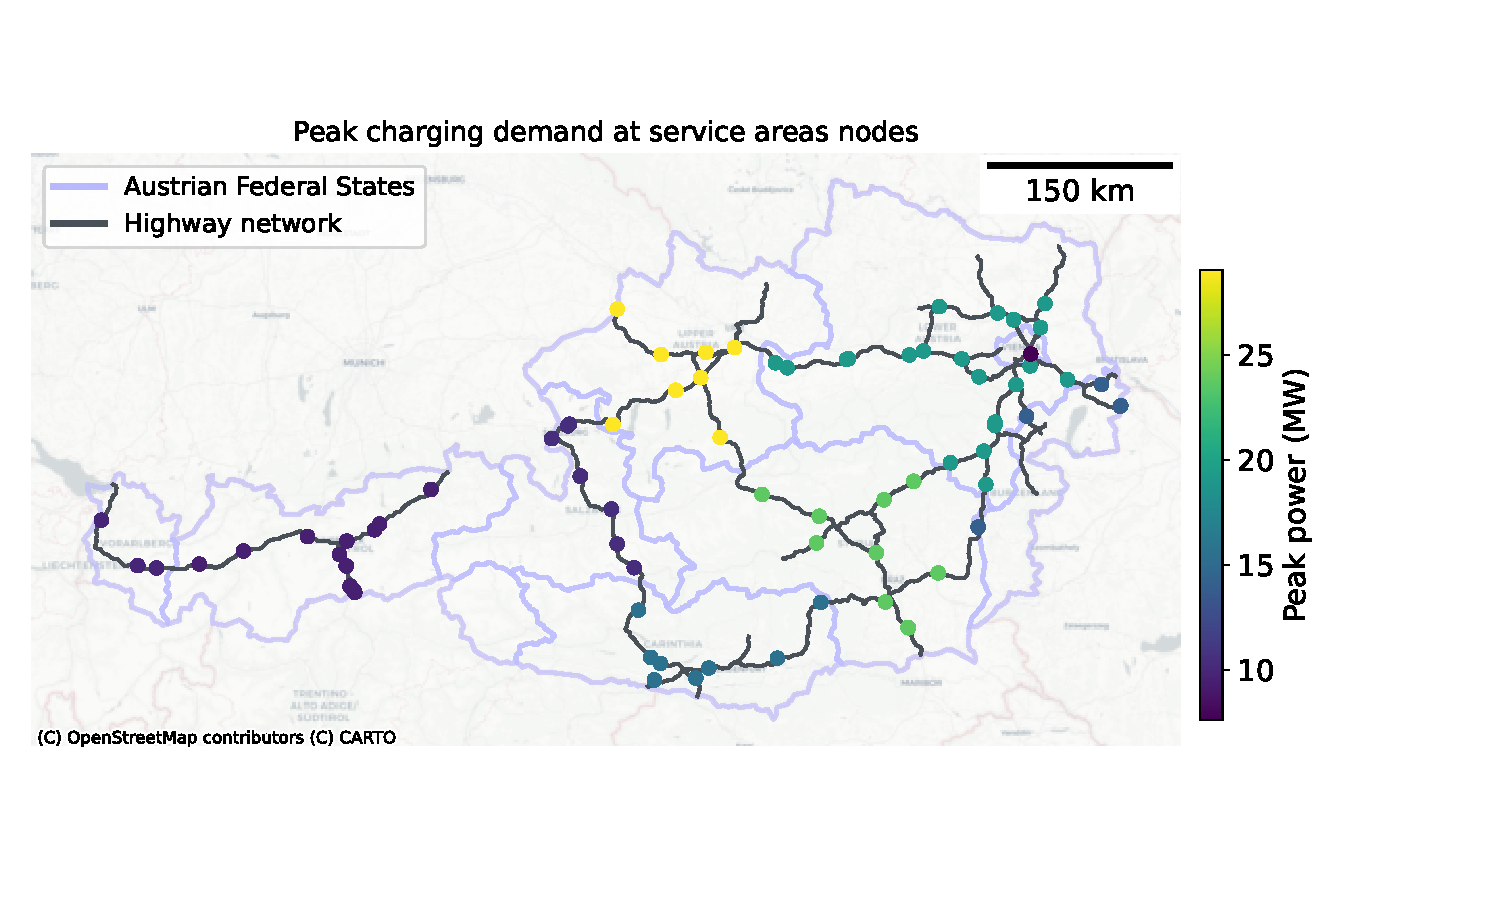
\includegraphics[width=0.9\textwidth]{graphics/peak_demand_service_areas.pdf}
        \caption{ Approximation of charging peaks at Austrian resting areas for an 100\% electrified commercial vehicle fleet (positions retrieved from \cite{ASFINAG})}
        \label{fig:truck_highway_charging_peak}
    \end{figure}
     % Please add the following required packages to your document preamble:
% \usepackage{graphicx}
\begin{table}[H]
\centering
\caption{Annual charging demand of three different considered fleet types under different assumptions on electrification rate for the commercial vehicle fleet in Austria in 2040.}
\label{tab:results_charging_load}
\resizebox{\textwidth}{!}{%
\begin{tabular}{llrrcrrr}
\hline
                & \multicolumn{7}{c}{Total annual demand of fleet types 2040 (TWh)}                                                                       \\ \cline{3-8} 
                & \textbf{Total}                    & \multicolumn{1}{c}{LDV} & \multicolumn{1}{c}{Bus} & \multicolumn{4}{c}{HDV}                      \\ \hline
                &                                   & \multicolumn{1}{l}{}    & \multicolumn{1}{l}{}       & \multicolumn{3}{c}{Charging location} &      \\ \cline{5-7}
Scenario &  & \multicolumn{1}{l}{} & \multicolumn{1}{l}{} & Depot & \multicolumn{1}{c}{Highway (day time)} & \multicolumn{1}{c}{Highway (night time)} & Total \\ \cline{5-8} 
\textit{LOW}    & \multicolumn{1}{r}{\textbf{7.4}}  & 2.7                     & 1.3                        & \multicolumn{1}{r}{1.8}  & 1.1  & 0.5 & 3.4  \\
\textit{MEDIUM}   & \multicolumn{1}{r}{\textbf{9.6}}  & 2.7                     & 1.3                        & \multicolumn{1}{r}{3.1}  & 1.7  & 0.8 & 5.6  \\
\textit{HIGH} & \multicolumn{1}{r}{\textbf{15.2}} & 2.7                     & 1.3                        & \multicolumn{1}{r}{6.2}  & 3.5  & 1.5 & 11.2 \\ \hline
\end{tabular}%
}
\end{table}
        \begin{figure}[H]
            \centering
            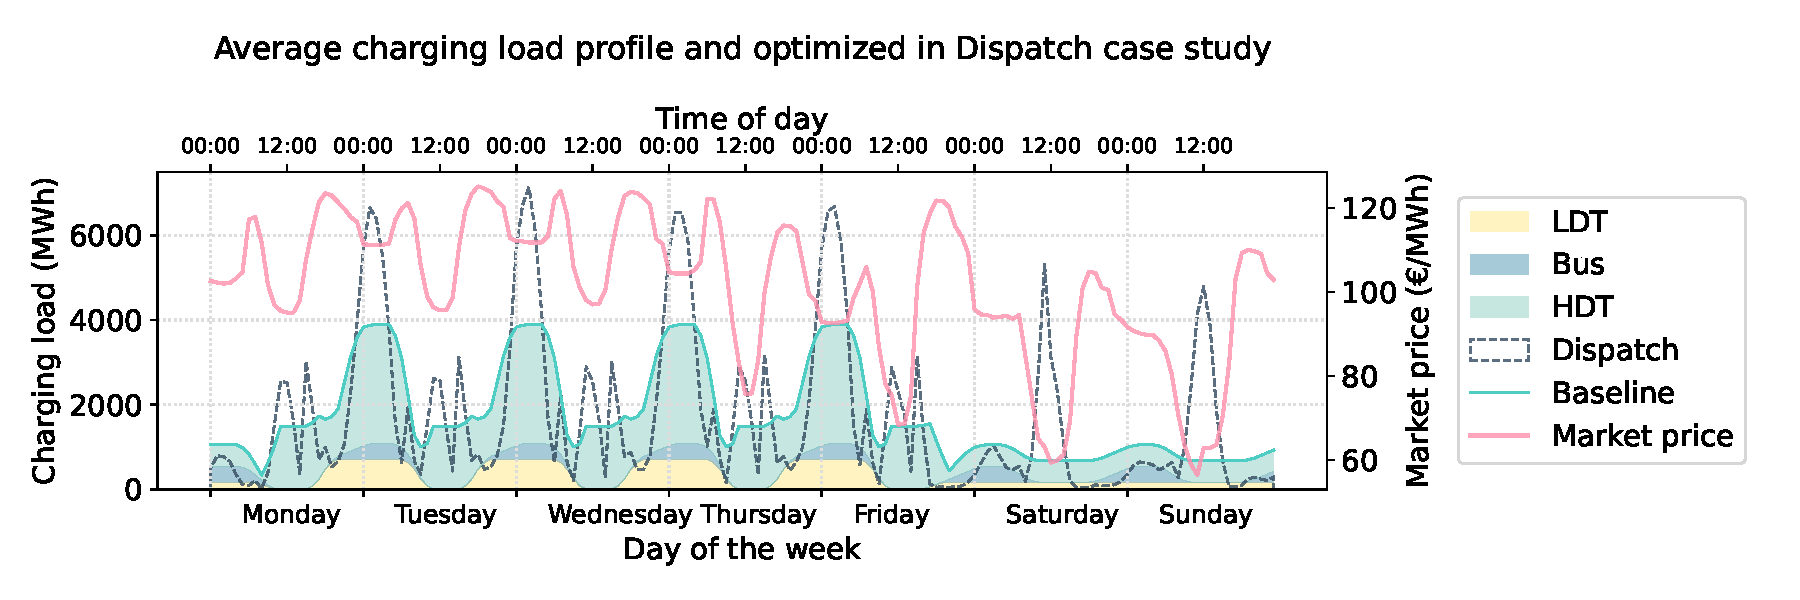
\includegraphics[width=1\textwidth]{graphics/average_load_profile_dispatch.pdf}
            \caption{Aggregated charging demand profile of the commercial \ac{BEV} fleet in the \textit{Baseline} and \textit{Dispatch} case study with the average day-ahead market price.}
            \label{fig:dispatch_time}
        \end{figure}
    
    \subsection{Impact of the market participation of the commercial \ac{BEV} fleet in dispatch}
        Figure \ref{fig:dispatch_time} further indicates the shifted charging demand as a result of the dispatch optimization, i.e. when the charging processes is aggregated and centrally coordinated to achieve minimum costs for dispatch. The red line indicates the average electricity market price in Austria. During work days, two price lows are identified to be around noon and around midnight. These coincide with the peaks of charging demand which increase the night peak during weekdays by 80\% from the \textit{Baseline} charging profile. During the weekends, significant price lows appear during noon and create a peak load value that is roughly eight times greater than the \textit{Baseline} charging demand value at this hour. 

        Figure \ref{fig:annual_dur_curve} shows the impact of the application of the market participation of the commercial \ac{BEV} fleet on the total electricity load in Austria in 2040. The price-oriented charging coordination increases peak load values by up to 24 \% compared to the \textit{Baseline} case study and decreases the load during hours of lower values. 

        \begin{figure}[H]
            \centering
            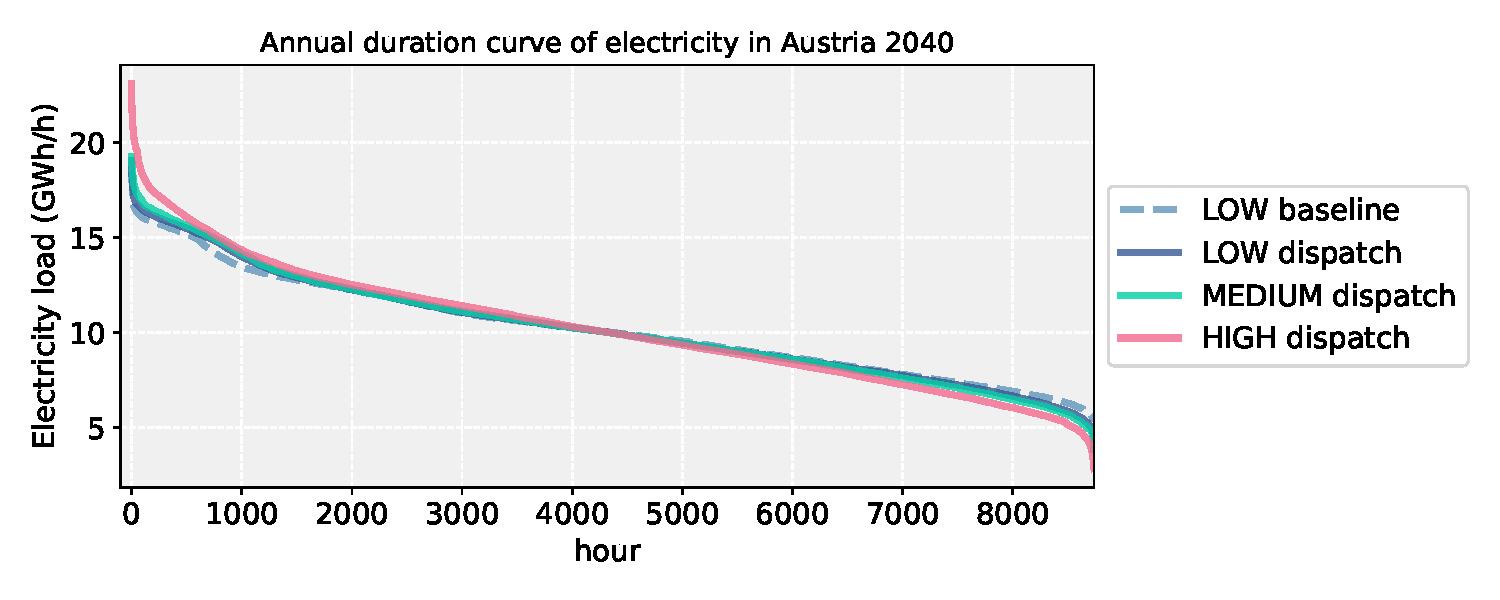
\includegraphics[width=0.9\textwidth]{graphics/annual_duration_curve.pdf}
            \caption{Annual duration curve of electricity demand in Austria in 2040 for different case studies and electrification scenarios.}
            \label{fig:annual_dur_curve}
        \end{figure}

        % What is evident here?
        % \begin{itemize}
        %     \item night-time peak 
        %     \item some flexibility at service areas
        %     \item extremly increased peaks during day time at weekends (by \dots \%)
        % \end{itemize}

        
        % \begin{itemize}
        %     \item transition here smoothly to the temporal shift. 
        %     \item dispatch: response to market price: high nicht peaks and mid-day peaks (display with electricity prices)
        %     \item redispatch: shift is lower
        %     \item annual duration curve: increase in peak demand
        %     \item costs: substantial increase in dispatch costs, but its application in redispatch decreases redispatch costs
        % \end{itemize}



    
    % \begin{itemize}
    %     \item Individual load profile; change in load curve!; potential benefit in electricity costs for fleet owners? geographic distribution of used re-dispatch? where and which location and of which fleet type?
    %     \item 
    % \end{itemize}

    % \hl{What outputs do we have of this analysis? what might be interesting to show in the results?}
    %     \begin{itemize}
    %     \item Contrary behavior between prices and demand: price convergence and demand peak divergence
    %     \item Rsults of the traffic flow model: Why it is important to consider the spatial distribution of flexibility? E.g. transferable to balancing and ancillary service market -> see SOTA
    % \end{itemize}
    
        % \begin{itemize}
        %     \item \textbf{Figure 1}: Temporal load distribution, stacked area plot with color indication per fleet type, accumulated on whole Austria --- including e-truck highway vs. depot 
        %     \item \textbf{Figure 2}: Load and flexibility by charging location (barplot)
        %     \item \textbf{Figure 3}: Geographic differences in temporal load shift at the 17 nodes (Wh)
        %     \item \textbf{Figure 4}: Geographic distribution of peak capacities. Highways + depots. (W/km2 u. W/Raststation)
        % \end{itemize}
        \subsection{Spatial differences in participation in redispatch measures}
        Figure \ref{fig:redispatch_time} displays the annual average for a week of the resulting charging demand profile from the participation of the commercial \ac{BEV} fleet in congestion management aggregated for Austria. The resulting load peaks are significantly lower than in the \textit{Dispatch} case study and, on average, these do not significantly exceed the levels of the \textit{Baseline} load profile. On weekend days, the charging load is shifted, similarly as in the \textit{Dispatch} case, to around noon, increasing the \textit{Baseline} load by 68\%. 
        While for the dispatch calculations, the charging processes are aggregated to the bidding zone level, the geographic variations are particularly relevant to the redispatch modeling where the topology of the transmission grid, and geographically varying dispatch and load centers are important factors. Figure \ref{fig:shifted_load_profiles} displays average weekly charging profiles at all nodes representing the Austrian transmission grid. Compared to the average aggregated load profile displayed in Figure \ref{fig:redispatch_time}, significant variations are visible in the absolute magnitude of the load profile and also in the shape of the curves. This is due to two reasons: (1) the region-specific scaling of charging profiles for different fleet types, (2) the region-specific usage of the charging flexibility. Three profiles are highlighted in Figure \ref{fig:shifted_load_profiles} and here indicated with yellow (\textit{Node A}), red (\textit{Node B}) and blue (\textit{Node C}). These nodes are selected because of distinct differences between the shapes of the charging profiles. With the selection of these nodes, the goal is to further elaborate on the causes for these differences. Figure \ref{fig:node_allocations} indicates the respective positions of these nodes. \textit{Node A} and \textit{Node B} are nodes allocated in the Northeast of Austria, \textit{Node C} in the South, near the boarder to Italy. The \textit{Baseline} charging profiles and the average \textit{Redispatch} profiles are displayed in Figure \ref{fig:selected_nodes_profiles}.
        
        \textit{Node A} is allocated in the Austrian Federal State called \enquote{Lower Austria}. It is the Federal state with the second-highest population number and the biggest area. Further, Lower Austria is the state with the highest total kilometers of highway and motorway network. In the charging profile (Figure \ref{fig:selected_nodes_profiles}), relatively high daytime peak loads are visible. When the commercial \ac{BEV} fleet participates in the redispatch measures, the charging profile does not significantly deviate from the \textit{Baseline} profile. However, the absolute peaks during noon on the highway, as well as at night around midnight, increase. A similar peak as in Figure \ref{fig:redispatch_time} on the average Saturday appears. 
        \textit{Node B} is positioned in the Austrian capital, Vienna, which has the highest population and population density as it consists of almost exclusively urban area. This is reflected in the high amount of charging demand by light-duty trucks (see Figure \ref{fig:selected_nodes_profiles}) and the lowest day-time demands for charging at service areas. Similarly as for \textit{Node A}, no significant deviations to the \textit{Baseline} profile are observed. In contrast to this, in \textit{Node C}, the shape of the charging profile is significantly altered when the commercial \ac{BEV} fleet is participating in redispatch measures. During work days, the charging load of the night time is significantly shifted to earlier times. During the weekend, load peaks are present around 6 pm. 
        \begin{figure}[H]
            \centering
            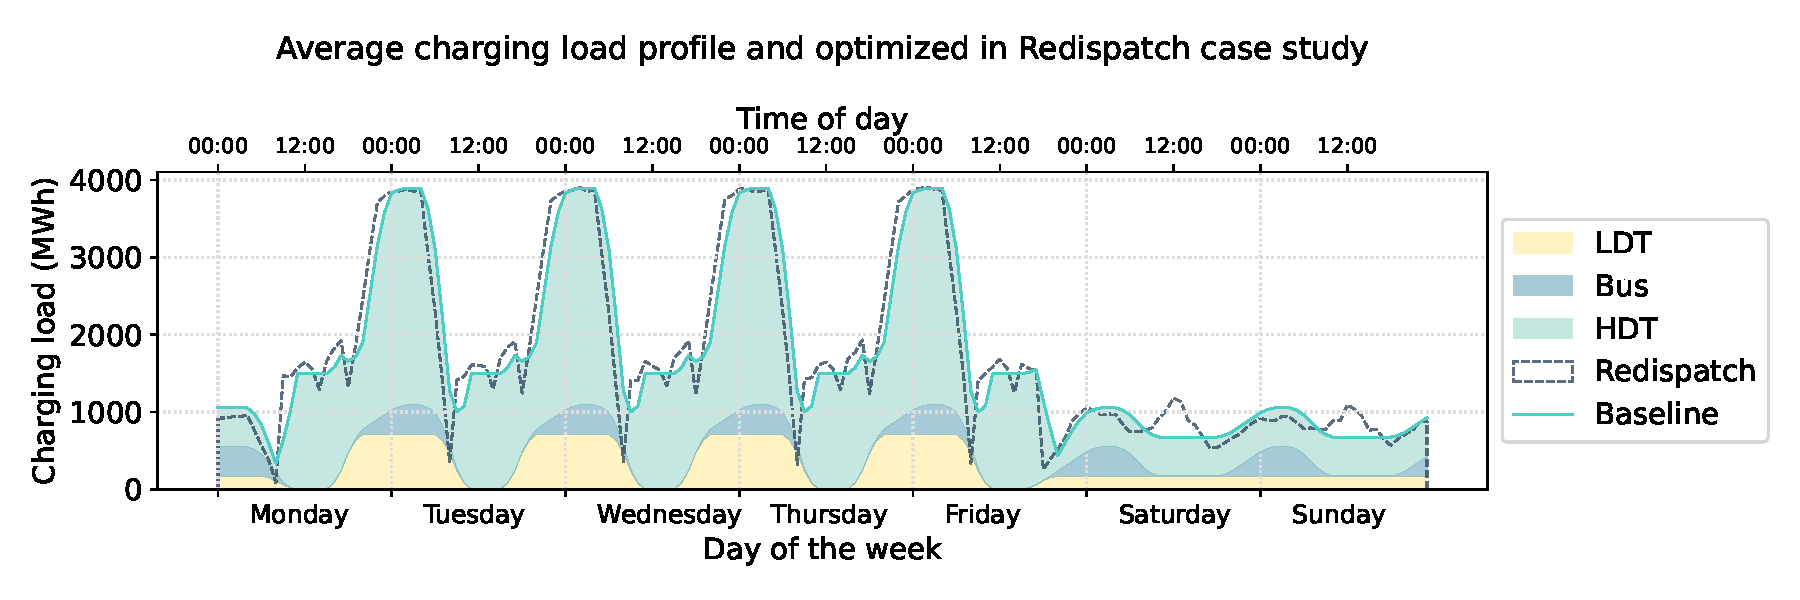
\includegraphics[width=1\textwidth]{graphics/average_load_profile_redispatch.pdf}
            \caption{Aggregated charging demand profile of the commercial \ac{BEV} fleet in the \textit{Baseline} and \textit{Redispatch} case studies.}
            \label{fig:redispatch_time}
        \end{figure}


        \subsection{Comparison of redispatch costs}

        Figure \ref{fig:costs} compares the redispatch costs for all case study and electrification scenarios. These are the core observations:
        \begin{itemize}
            \item In the \textit{Baseline} case study, the increasing electrification of the commercial fleets has a limited impact on the costs of dispatch measures. The costs decrease slightly by 4M\euro, between the \textit{LOW} and \textit{HIGH} scenario.  
            \item In contrast to this, the increasing electrification of the truck fleet does affect the redispatch costs substantially when the flexibility is utilized in the dispatch. At the electrification rate of 30\% of \ac{HDT} fleet, costs increases by around 40\% between the initial charging strategy and the coordination with dispatch. 
            \item The coordination of the charging profiles regarding the minimization of the redispatch costs effectively decreases the redispatch costs by about 30-35\% to the \textit{Baseline} case. 
        \end{itemize}
        




       \begin{figure}[H]
            \centering
            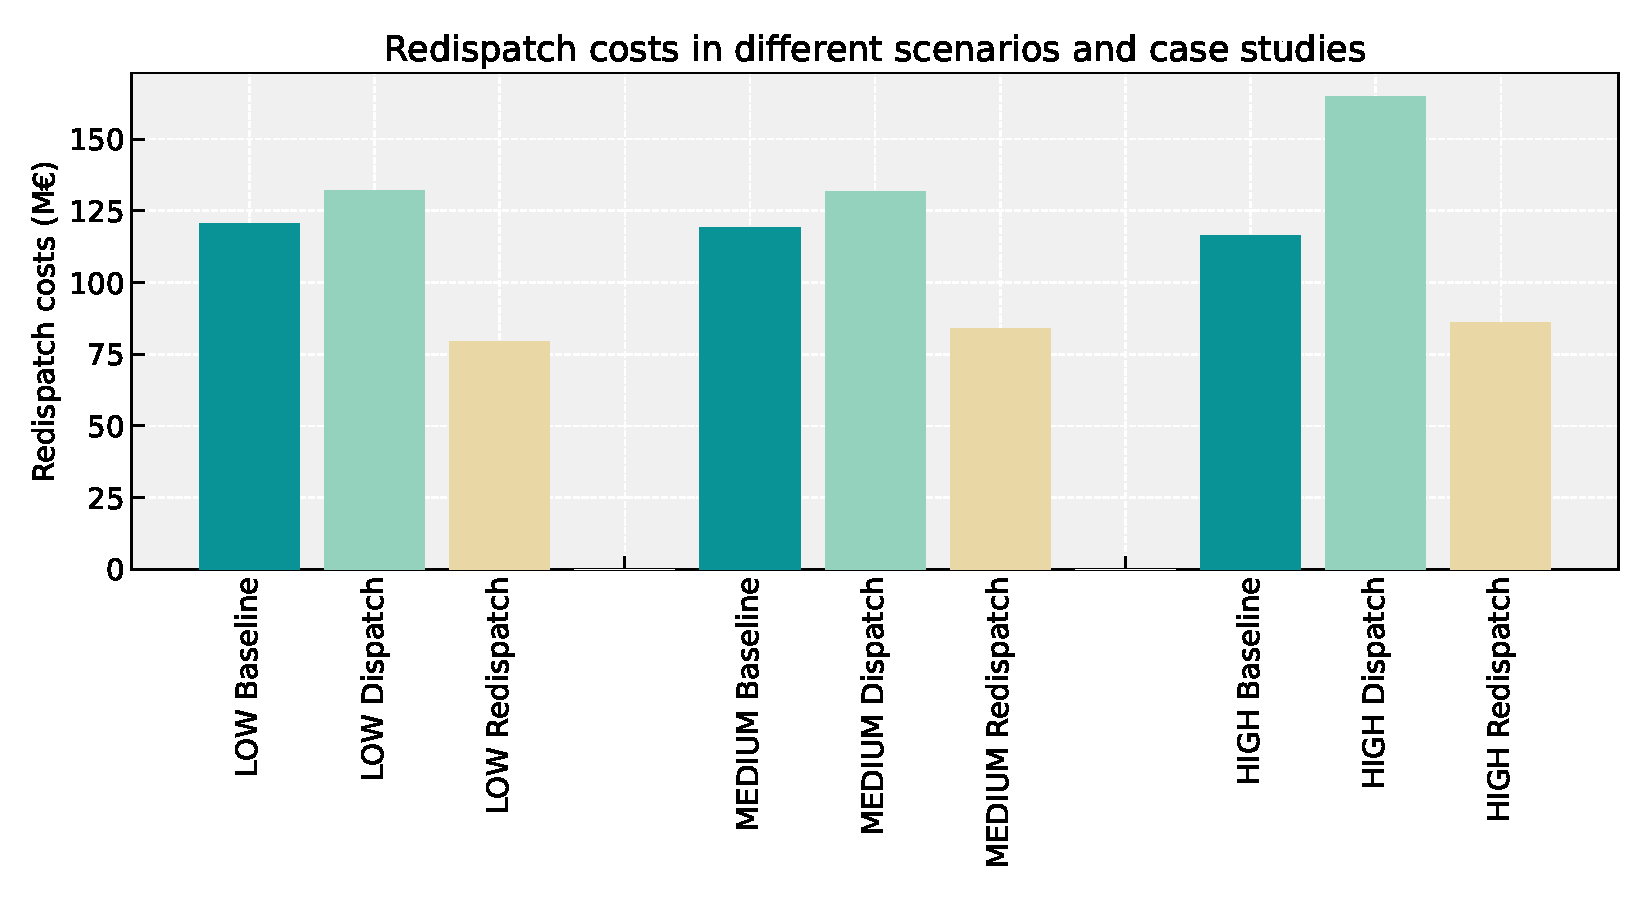
\includegraphics[width=0.8\textwidth]{graphics/costs.pdf}
            \caption{Cost comparison of redispatch costs for different scenarios and case studies for 2040.}
            \label{fig:costs}
        \end{figure}

        \begin{figure}[H]
            \centering
            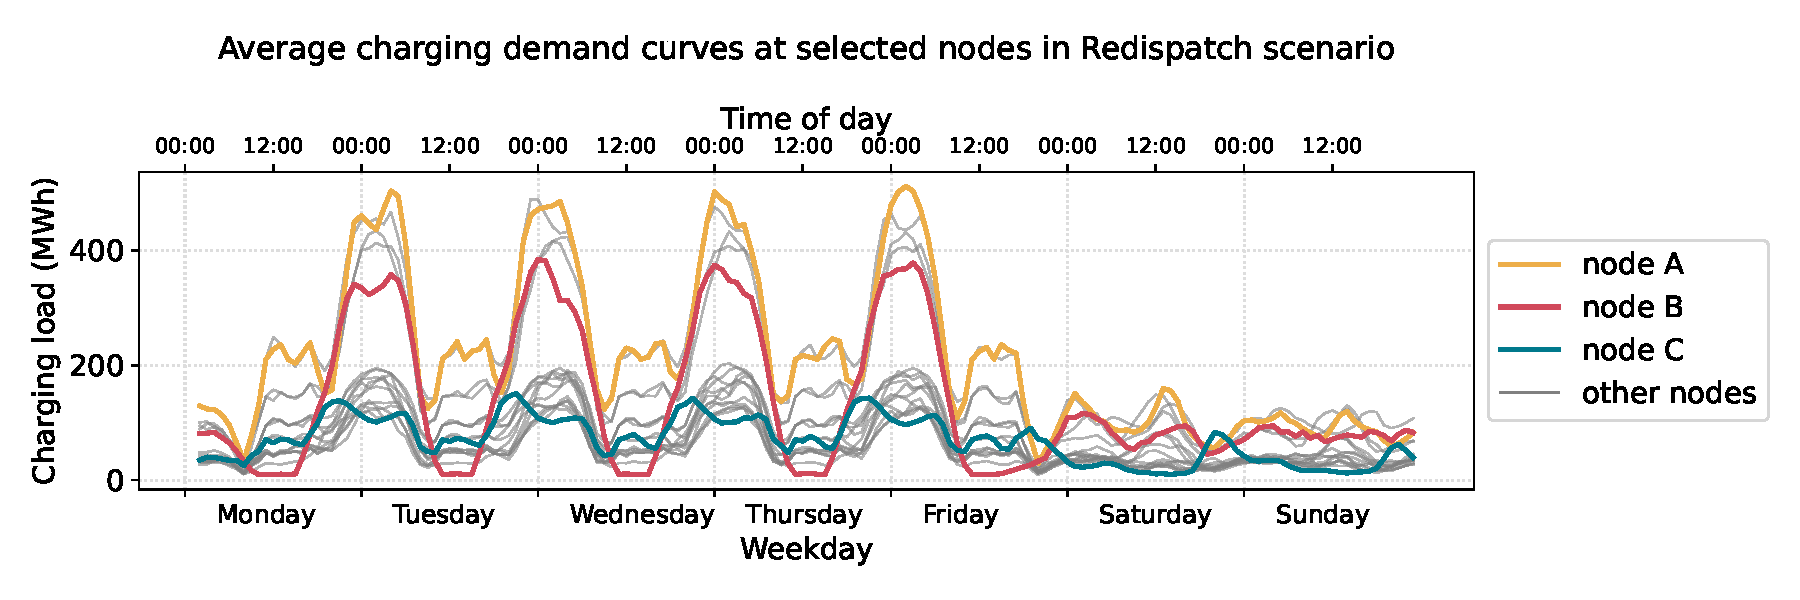
\includegraphics[width=0.9\textwidth]{graphics/shifted_load_profiles.pdf}
            \caption{Charging load curves resulting from participation of the commercial \ac{BEV} fleet in redispatch at different nodes in the transmission grid.}
            \label{fig:shifted_load_profiles}
        \end{figure}

        \begin{figure}[H]
            \centering
            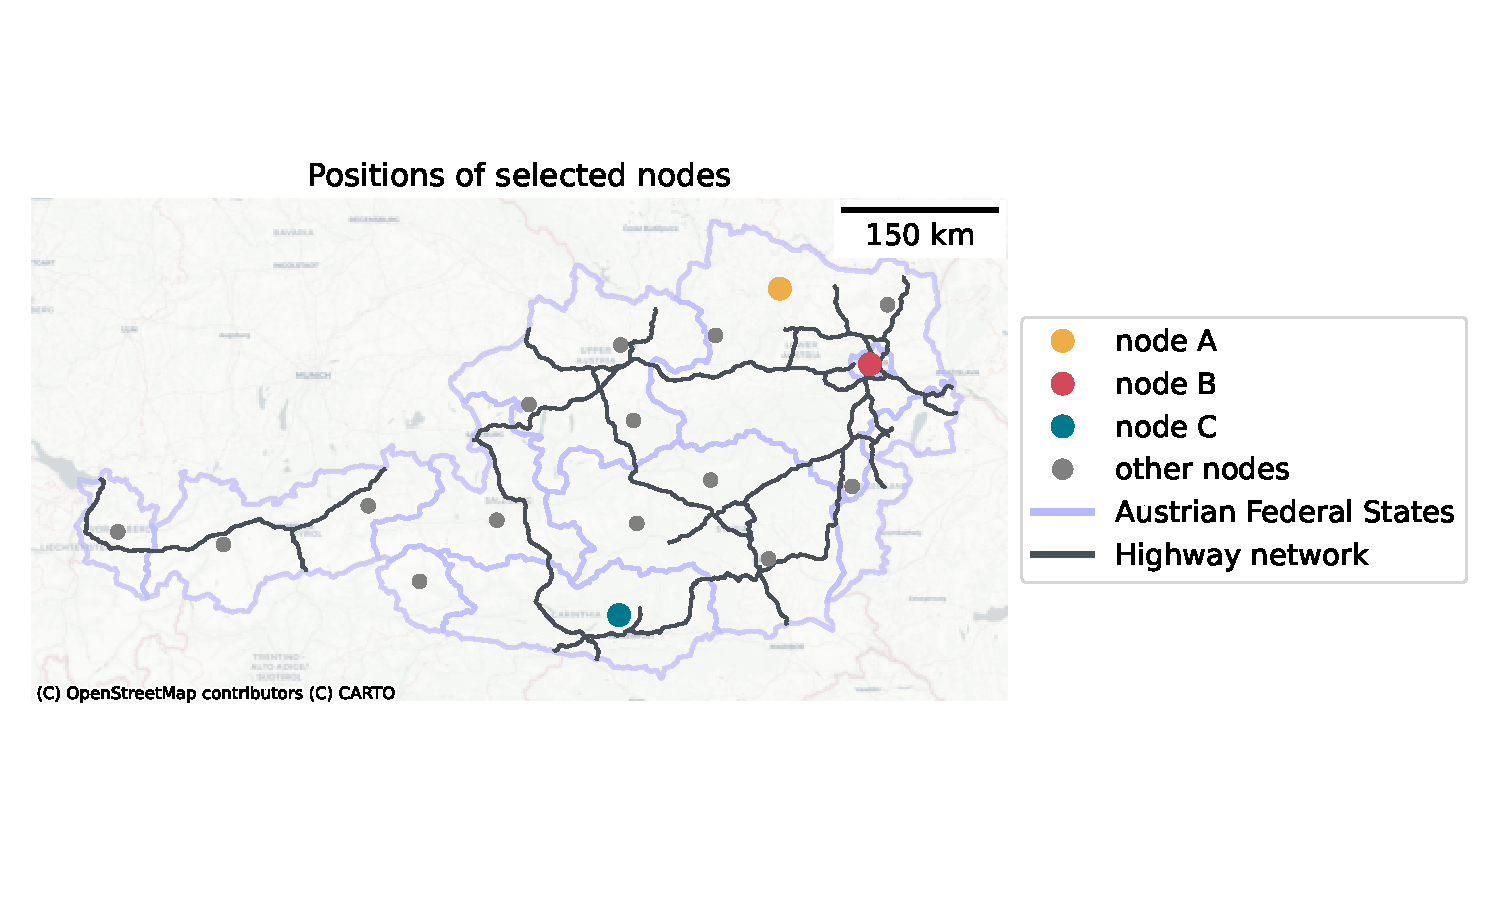
\includegraphics[width=0.9\textwidth]{graphics/selected_nodes.pdf}
            \caption{Geographical allocation of selected nodes representing the Austrian transmission grid in the redispatch model.}
            \label{fig:node_allocations}
        \end{figure}

        % \begin{figure}[H]
        %     \centering
        %     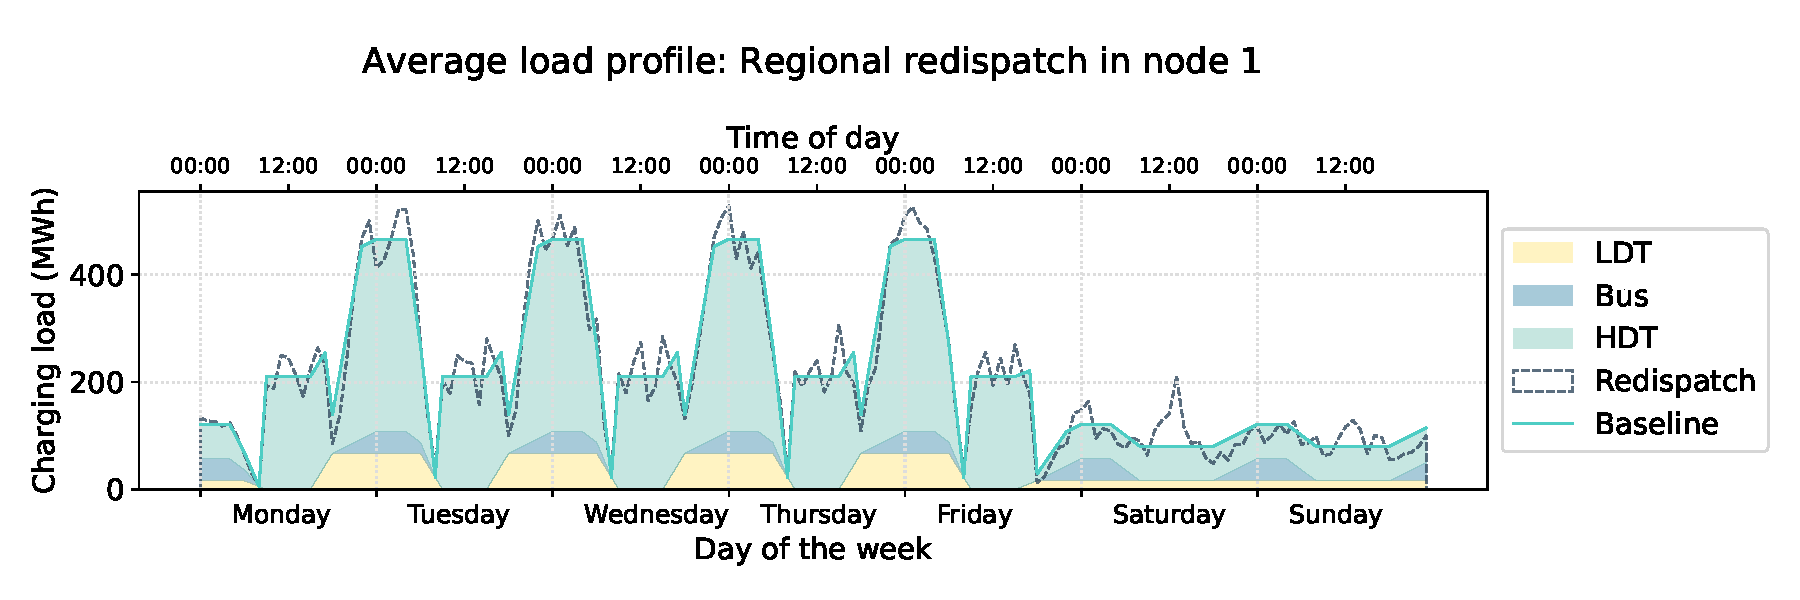
\includegraphics[width=0.9\textwidth]{graphics/NOEaverage_load_profile.pdf}
        %     \caption{Node 1: Charging profile in the \textit{Baseline} case and in the charging profile as a result of the application of smart charging in redispatch measures.}
        %     \label{fig:node1_shift}
        % \end{figure}

        % \begin{figure}[H]
        %     \centering
        %     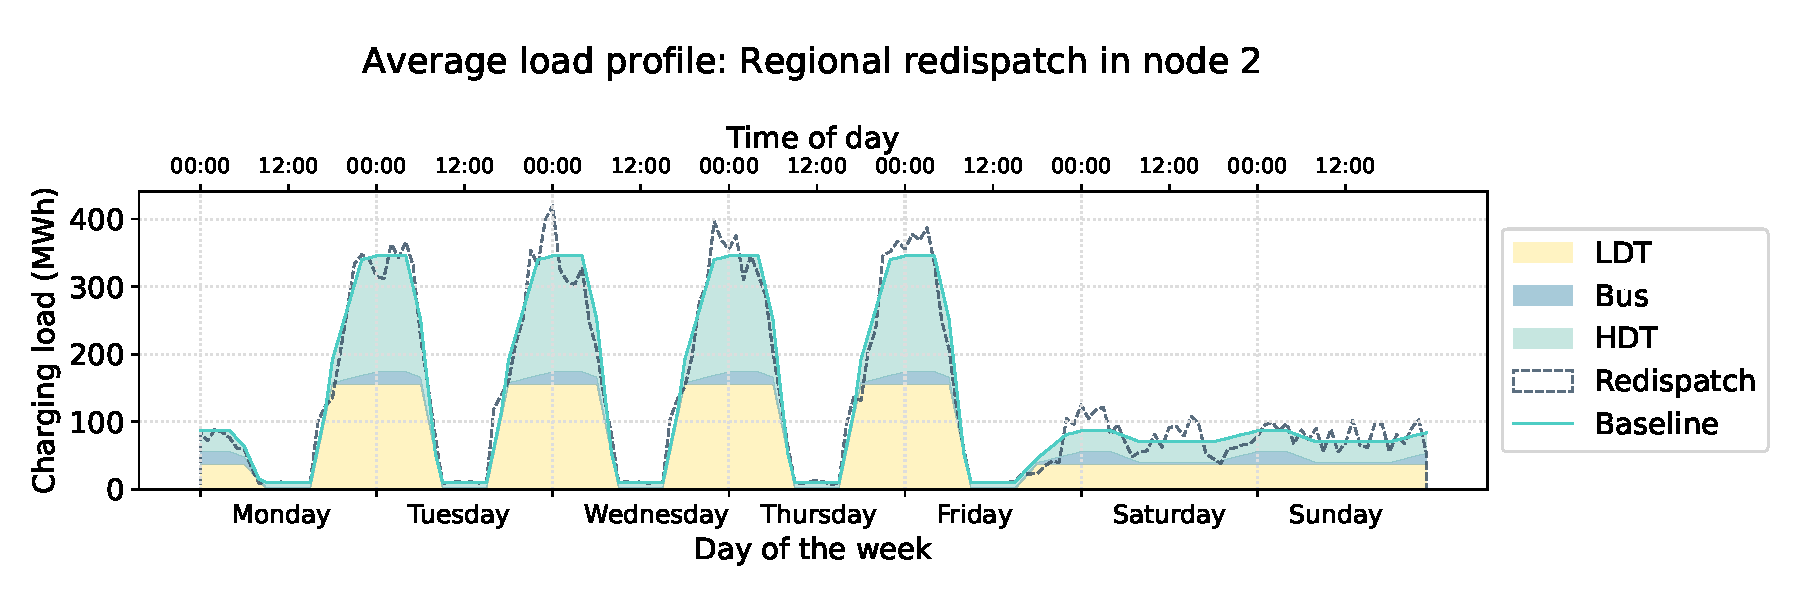
\includegraphics[width=0.9\textwidth]{graphics/Waverage_load_profile.pdf}
        %     \caption{Node 2: Charging profile in the \textit{Baseline} case and in the charging profile as a result of the application of smart charging in redispatch measures.}
        %     \label{fig:node2_shift}
        % \end{figure}
        
        % \begin{figure}[H]
        %     \centering
        %     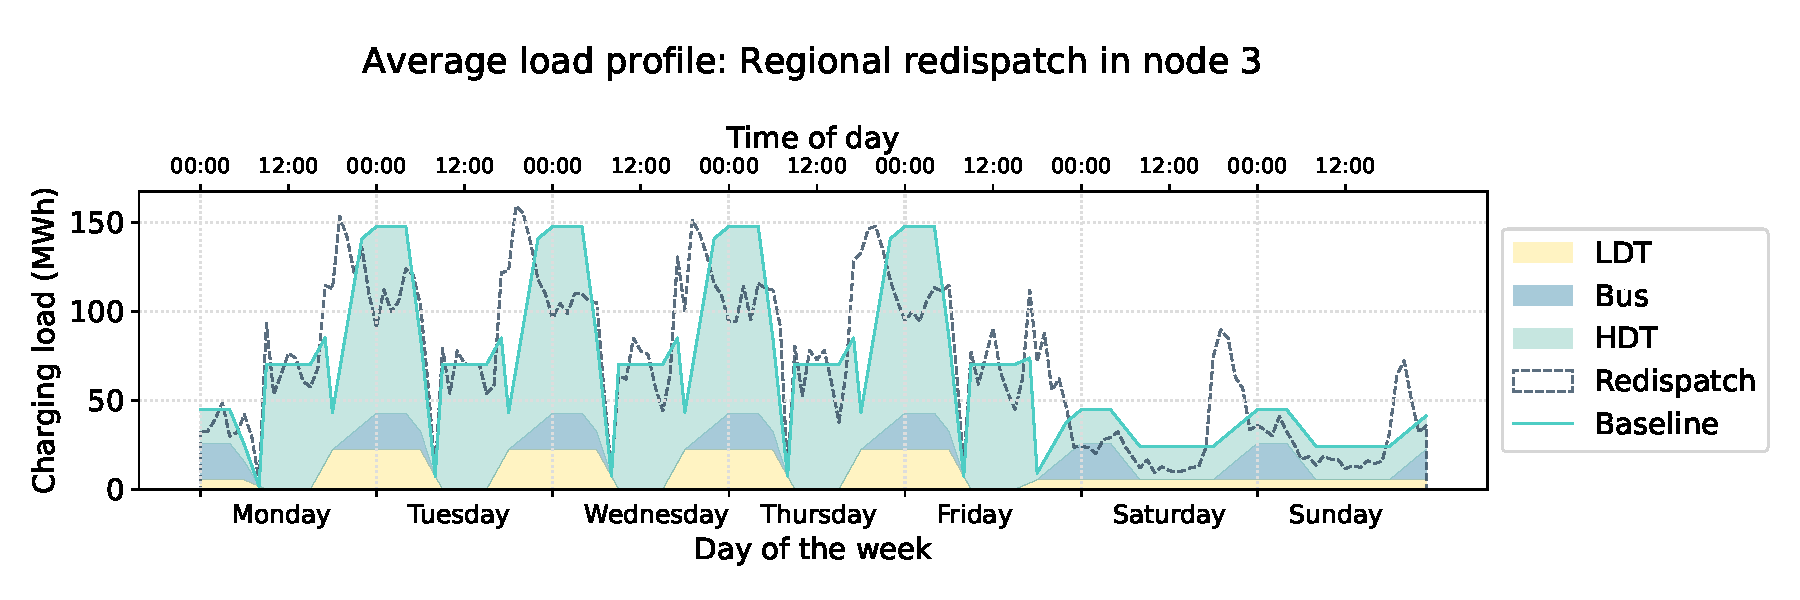
\includegraphics[width=0.9\textwidth]{graphics/KTN_waverage_load_profile.pdf}
        %     \caption{Node 3: Charging profile in the \textit{Baseline} case and in the charging profile as a result of the application of smart charging in redispatch measures.}
        %     \label{fig:node3_shift}
        % \end{figure}
    \begin{figure}[H]
    \centering
    
    % First subfigure
        \centering
            \begin{minipage}[t]{1\textwidth}
            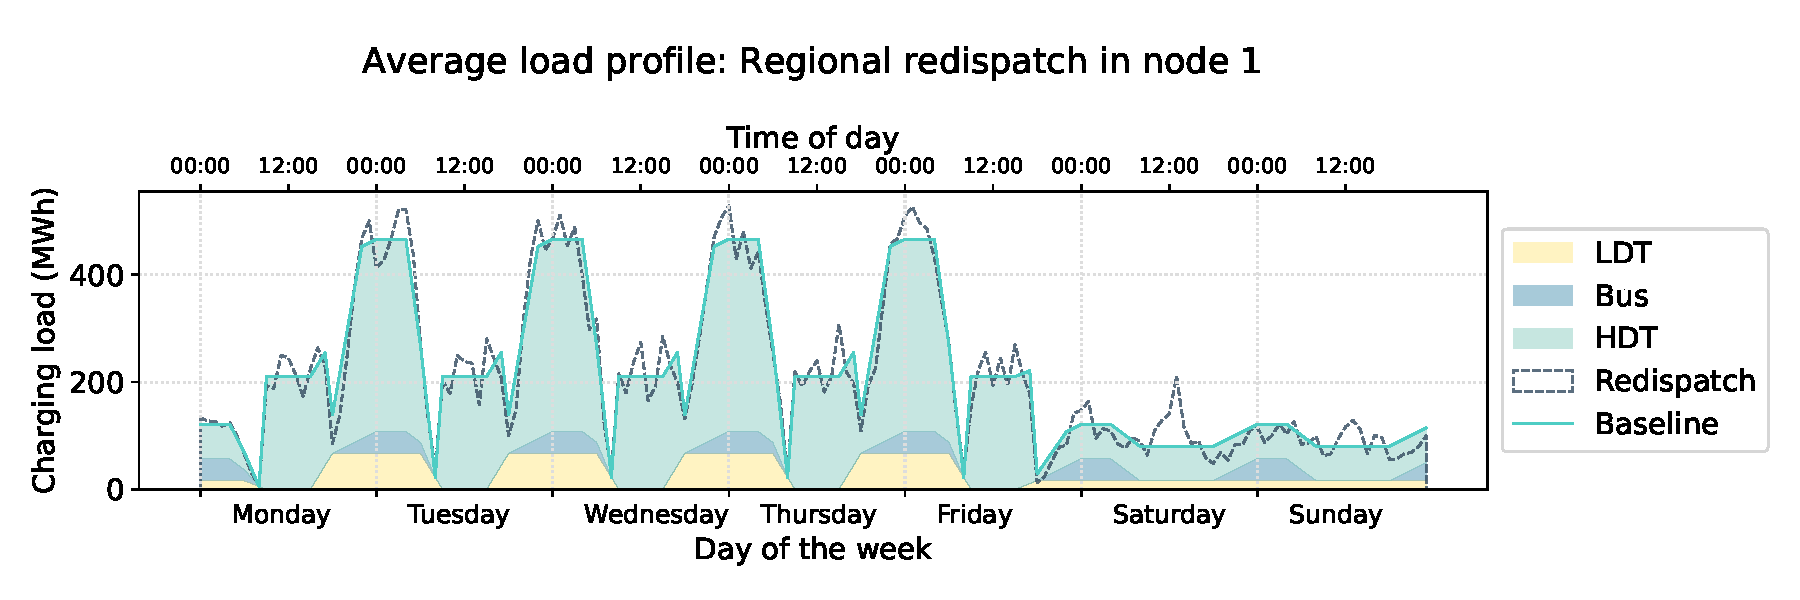
\includegraphics[width=\linewidth]{graphics/NOEaverage_load_profile.pdf}
            \label{fig:subfig1}
            \end{minipage}%
        \hfill
    % Second subfigure
    \begin{minipage}[t]{1\textwidth}
        \centering
        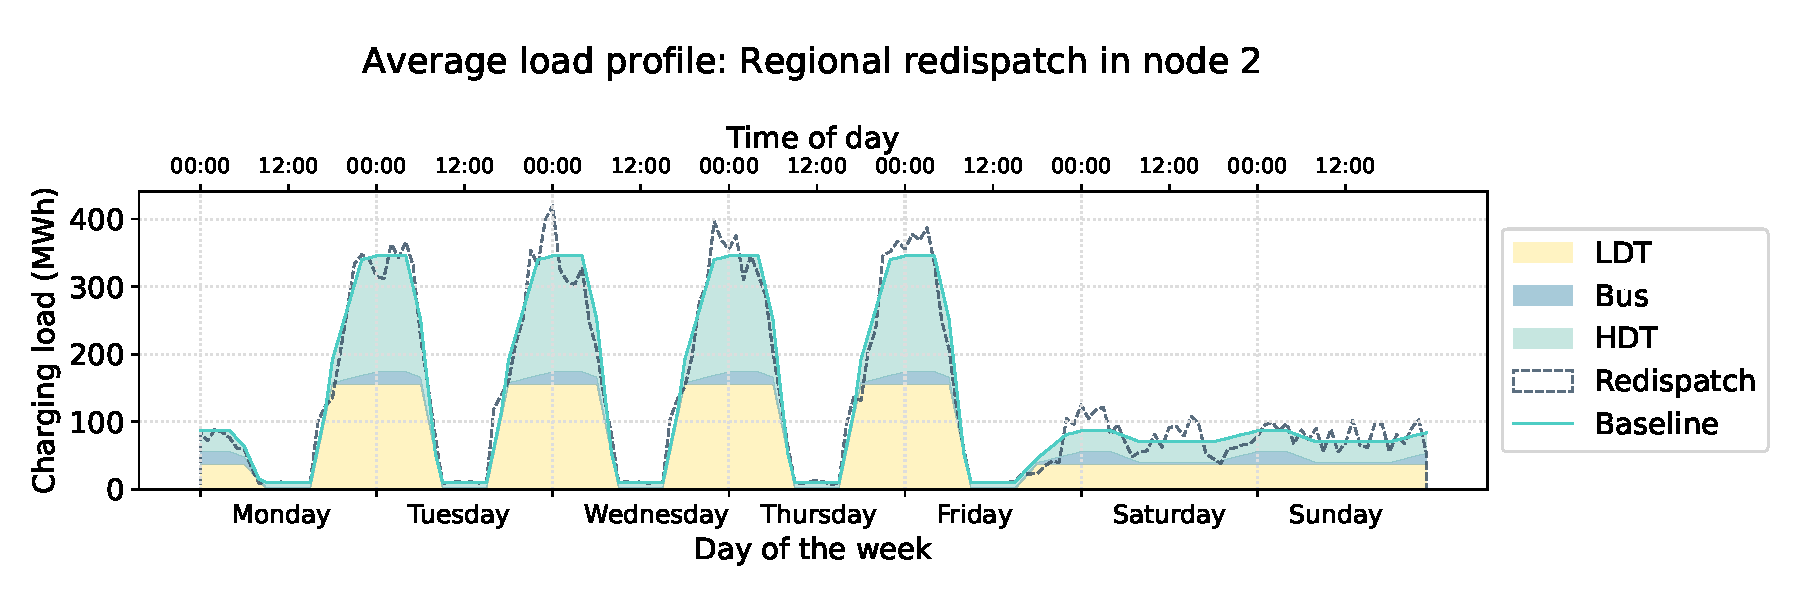
\includegraphics[width=\linewidth]{graphics/Waverage_load_profile.pdf}
        \label{fig:subfig2}
    \end{minipage}
    \hfill
    % Third subfigure
    \begin{minipage}[t]{1\textwidth}
        \centering
        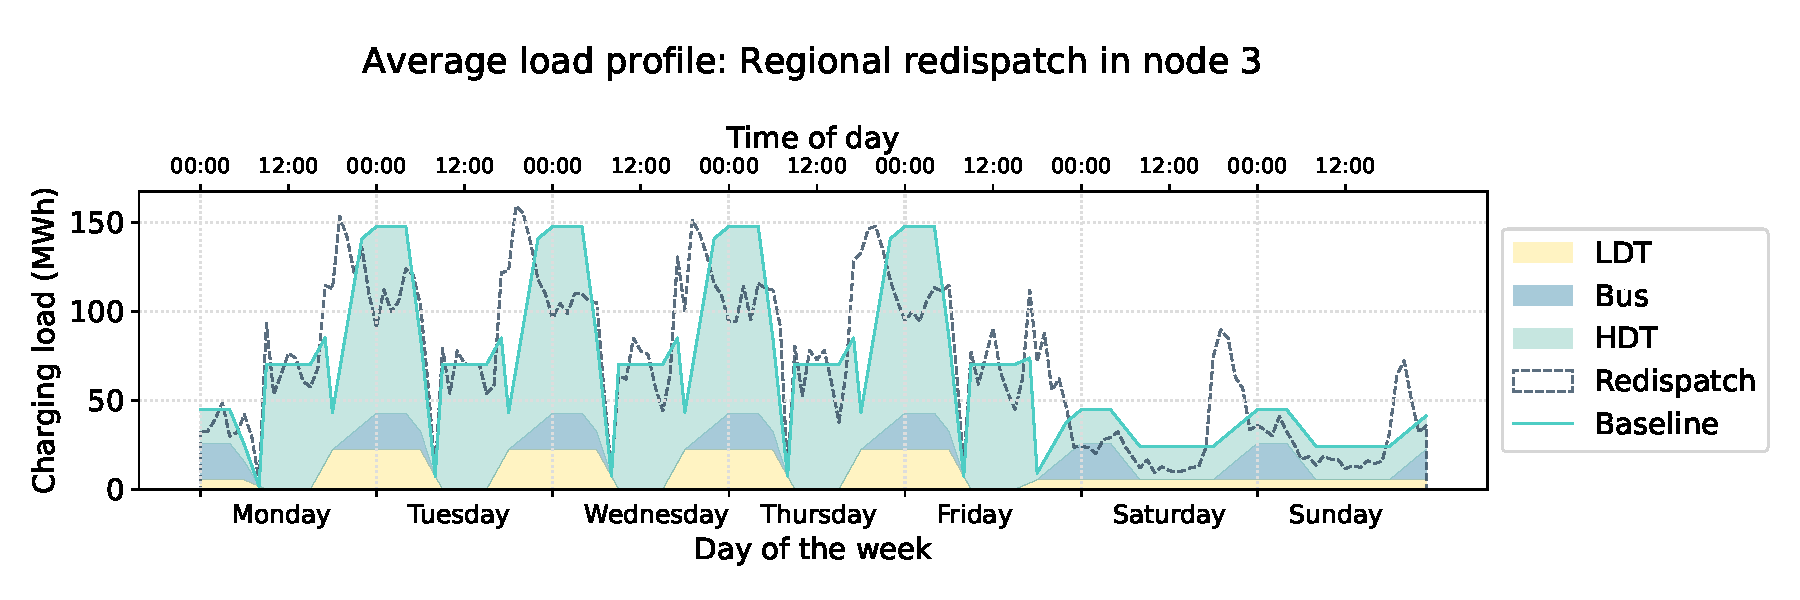
\includegraphics[width=\linewidth]{graphics/KTN_waverage_load_profile.pdf}
        \label{fig:subfig3}
    \end{minipage}
    
    \caption{Average load profile in three selected node for case studies \textit{Baseline} and \textit{Redispatch}.}
    \label{fig:selected_nodes_profiles}
\end{figure}

\section{Discussion}
        \subsection{Spatio-temporal distribution of commercial \ac{BEV} fleet charging demand}
            
            While the magnitude of \ac{LDT} and bus charging demand is modeled based on features of the regions itself, such as the total population, the \ac{HDT} charging demand is modeled based on traffic flow data. This allows us to model the charging demand of trucks bottom-up and to differentiate between charging demand to be covered en-route and in depots at the origin and destination regions. The benefit of this approach is evident given the substantial differences in the load distribution observed between Austrian regions, as well as by the dominance of \ac{HDT} charging demand in the accumulated charging demand of the commercial \ac{BEV} fleet.    

            The temporal distribution of the charging load is deducted from the assumption of down times and of the charging strategy. In the present paper, we have assumed that charging at highway charging stations would be a preferred charging strategy for \ac{HDT}s that are required to take a break en route. This may lead to an overestimation of the daytime load at service areas. However, we did not count in trucks that would exclusively be able to charge publicly during day time due to the lack of available depot charging of the trucking fleet operators. Our results indicate that this daytime charging is substantial in most regions of Austria, while the highest demand peaks are allocated at nighttime. During the weekend, the charging load is moderate and provides extensive flexibility given that for the recharge at weekends, the charging capacity of similar magnitude as during the week is available. \added{It must be noted here that these increased charging load peaks may be overestimated due to neglecting costs for the activation of the flexibility provided by the commercial fleet and, further, assuming the participation of the entire commercial vehicle fleet in the centrally coordinated charging. However, the results related to the different degrees in the electrification of the commercial fleet can be transferred to different magnitudes in the participation in the charging coordination.}      
            % The highest peak loads of commercial charging are allocated in the North-East of Austria, which also coincides with the current electricity load distribution. While looking at the temporal dimension, there is a high contrast in demand peaks during the daytimes and night times, depending of whether the node is associated with a region of big area and the population density. 
            % The usage of the traffic flow data to determine HDT charging demand provides information that is not directly determined by the local population number but related to the allocation of highway infrastructures and the origin and destination points of trucks that these connect. 
    
            % The consideration of the HDT traffic flows also gives insights into the spatially varying power requirements for service areas which also depend on the density of available service areas along the highway segments. The day peak power levels for service areas have been detected in a region that is directly next to a region in which the highest charging load at depots is allocated, i.e. indicating that this is a frequent origin/destination region for HDT routes.  

        \subsection{Impact on redispatch costs}
            The utilization of the commercial \ac{BEV} fleet charging flexibility in the day-ahead market clearing shifts the load from off-peak times to peak times and introduces a substantial increase grid congestion due to the neglection of the transmission grid topology in the dispatch optimization. Observing the time series of the average weekly charging profiles of the dispatch optimized charging together with the day-ahead market price, relatively high price volatility appears during weekends, and, due to the high charging flexibility on weekends, the initial charging profile is substantially altered. The activation of the demand-side flexibility of the charging processes is not weighted by any cost parameter in the dispatch objective and is exclusively limited in time by the plug-in times and in magnitude constrained by assumed charging capacities. This implies that if fleet operators coordinate the fleet charging market-price based, substantial peak loads occur and redispatch costs increase. To avoid this in the future, targeting regulatory incentives are needed-such as peak or dynamic pricing-and most importantly, these would also have to be dependent on the geographical allocation. The potential effectiveness of the latter is also supported by the location-dependent charging profiles resulting from the participation in the redispatch measures. 

        \subsection{Effect on charging processes by flexibility utilization in dispatch and redispatch markets}
            In the initial estimation of the charging profiles, all fleets are assumed to be charged at power levels that are constant and the lowest possible to cover the charging demand in their period of connection. This reduces the risk of rapid battery degradation. In the case of aggregated flexibility utilization in the dispatch, the power levels increase significantly which is less favorable for the long-term battery performance. When participating in redispatch measures, the differences between this charging profile and the initial charging strategy do not differ as drastically as in the case of participation in the dispatch and can be assumed to be more battery-life-time-friendly. 
    
            We have primarily assumed that the charging processes are limited to the downtime of the fleets. For highway charging, we introduced some flexibility in the timing of the break for truck drivers. Results imply that adapting the charging process market-price-based is more cost-efficient to avoid recharging around noon. Therefore, the trip would need to be started earlier or later than the average assumed departure time. This would impact the trip planning. \citeauthor{Scherrer2024Requirements} have found that the tour regularity varies greatly for individual vehicles and the need for the adaption of trip schedules to the timing of the charging process adds an additional layer of complexity to logistic planning \cite{Scherrer2024Requirements}. However, this needed adoption of trip patterns might not vary with the workday and season as our results do not show significant differences in the charging profiles between workdays and seasons. It is important to note here that this might be due to the modeling of exclusively one average week the entire year. Therefore, seasonal differences in traffic flow \added{that} occur due to f.e. holidays, as well as differences in the charging demand due to temperature-dependent energy consumption \added{are, hereby, neglected}. Additionally, these differences are further dependent on the allocation of the route. This is a particular challenge in the large-scale modeling of charging patterns as transport performance data is most times available aggregated for the period of one year. Further, operational patterns vary significantly in geography as this directly ties together with various socio-economic parameters that not only refer to the local region but also tie together interregionally. 


        \section{Conclusion and Future Work}

        The findings of this work extend the state of the art and give novel insights by quantifying the large-scale impacts of the electrification of light-duty trucks, heavy-duty trucks, and buses on the electricity system. Our results emphasize that with the increasing electrification of the transport sector, the cross-sectoral consideration of electricity and transport becomes increasingly important. The focal point of this cross-sectoral consideration must be the design of policy instruments to prevent increasing grid congestion and, in particular, to avoid large-scale aggregated charging in times of low market prices.
        This may encompass a strategic allocation of charging infrastructure by aligning the charging demand with locations of renewable energy sources while considering the requirements for charging infrastructure availability and reliability for commercial \ac{BEV} fleets. Moreover, an integrated view of the expansion of transport corridors and transmission grid expansion will gain importance in the long term. 
        
        % \textcolor{blue}{Ich würde hier einen Absatz schreiben mit Limitations, also was die Ergebnisse treibt, z.B. "It is important to note here that this might be due to the modeling of exclusively one average week the entire year.", etc. Dann ergibt sich ein smootherer Übergang zu Future Work.}
        It is important to note here that the underlying methodology for obtaining these insights has the main limitation that the annual charging profile is described by one average weekly profile. This may cause an overestimation or underestimation of the charging flexibility at certain times during the year. Therefore, we explicitly propose at least these two extensions of the methodology for future work:
        \begin{itemize}
            \item Considering seasonal differences in charging profiles will enhance the accuracy in the estimation of future charging profiles. This would extend the proposed modeling approach by considering seasonal fluctuations in charging demand due to the local temperatures affecting the battery performance and energy consumption due to heating or air conditioning in the vehicle. Further, charging demand may fluctuate depending on seasonal trends in transportation demand, for example, increased demand for the distribution of packages due to upcoming holidays, or differences in the transportation of cropped goods. The fluctuations in transportation demand may be particularly challenging as this is tied to further geographical differences, which are difficult to understand considering the availability of data on this. 
            \item While the temporal flexibility of charging has been considered in the present approach, the applied methodology does not consider the possibility of alternatively allocating the charging process in space. This is particularly relevant for vehicles that travel through multiple considered regions. This would allow us to further consider local differences in grid-friendly charging demand allocation and give insight into the design of effective pricing signals that are geographically variable. With this, the scope of analysis can also encompass the consideration of allocating the charging activity in different bidding zones showing effects of flexibility in times with a price divergence due to congestion. 
            % \item In regard to long-haul trucking, the allocation of charging processes in different market pricing zones within Europe would be of interest. This present analysis, on a larger scale, has the potential to explore how \ac{TSO}s and highway network operators of neighboring countries need to cooperate on this matter.
            
            % \item Next to the mentioned modeling extensions in the latter, the proposed framework has the potential to be used to study the effectiveness of different policy instruments related to relocating the charging demand in time and space in order to mitigate the increase in grid congestion. Particularly, \dots dynamic pricing? how to effectively incentives fleet operators while guaranteeing security in logistic operation
        \end{itemize} 
           % The spatial differences in charging profiles also emphasize the importance of the collaboration between highway network and transmission grid operators, and further also charging point and fleet operators, in the strategic allocation of charging infrastructure. On the one hand, this may contribute to reducing the magnitude of costs of redispatch and investments for reinforcement of grid infrastructures and, on the other hand, ensure cost-efficient and regulated operation of the commercial fleet. The coordinated and cross-sectoral planning and optimization need efficient methodologies to translate the complexities of traffic dynamics into effective indicators for the planning of the electricity system and allocation of transport-related infrastructures. 
 
        
        %% Use \subsubsection, \paragraph, \subparagraph commands to %% start 3rd, 4th, and 5th level sections.
%% Refer following link for more details.
%% https://en.wikibooks.org/wiki/LaTeX/Document_Structure#Sectioning_commands
\section*{Acknowledgments}
The authors acknowledge TU Wien Bibliothek for financial support through its Open Access Funding Programme.
\section*{Author contributions}
\textbf{Antonia Golab:} Conceptualization, Methodology, Software, Writing - Original Draft, Writing - Review \& Editing, Visualization \textbf{Christoph Loschan:} Conceptualization, Methodology, Software, Writing - Review \& Editing, Funding acquisition, Project administration \textbf{Sebastian Zwickl-Bernhard:} Conceptualization, Writing - Review \& Editing, Supervision \textbf{Hans Auer:} Conceptualization, Writing - Review \& Editing, Supervision, Funding acquisition

\bibliographystyle{elsarticle-num-names}
\bibliography{literature}
\newpage
\appendix



\section{Nomenclature}\label{sec:Appendix_nomenclature}
Decision variables in the \textit{Dispatch} model are used as parameters in the \textit{Redispatch} model.
% Please add the following required packages to your document preamble:
% 
% Please add the following required packages to your document preamble:
% \usepackage{graphicx}
\begin{table}[H]
\begin{tabular}{lll}
\textbf{Notation}                              & \textbf{Description}                                   & \textbf{Unit}              \\ \hline
\multicolumn{3}{l}{\textit{indices}}                                                                                                 \\ \hline
$t \in \mathcal{T}$                            & Time step                                              & h                          \\
$f \in \mathcal{F}$                            & Fleet type                                             &                            \\
$l \in \mathcal{L}$                          & Type of charging location (f.e. depot)                 &                            \\
$G_1 = (N_1, E_1)$                             & Charging network                                       &                            \\
$ n \in N_1, e \in E_1$                        &                                                        &                            \\
$G_2 = (N_2, E_2)$                             & Market prince zones                                    &                            \\
$ n \in N_2, e \in E_2$                        &                                                        &                            \\
$G_3 = (N_3, E_3)$                             & Transmission grid                                      &                            \\
$ n \in N_3, e \in E_3$                        &                                                        &                            \\
$ey \in \mathcal{EY}$                        & Electrolyzers                                          &                            \\
$fc \in \mathcal{FC}$                          & Fuel cells                                             &                            \\
$ps \in \mathcal{PS}$                          & Hydro storage units                                    &                            \\
$r \in \mathcal{RESE}$                         & Renewable energy sources                               &                            \\
${st} \in \mathcal{ST}$                        & Battery storage units                                  &                            \\
$th \in \mathcal{TH}$                          & Thermal power plants                                   &                            \\ \hline
\multicolumn{3}{l}{\textbf{Modeling of charging profiles}}                                                                  \\ \hline
$D^{\mathrm{BEV}}$ &
  Charging demand  &
  MWh \\
$\overline{D^{\mathrm{spec, BEV}}}$ &
  Average specific energy demand &
  MWh/km \\
$k$                                            & Number of vehicles                                     &                            \\
$R^f = \{R_1, R_2, \dots R_I\}$                & Routes of subfleets $i$ of fleet $f$                   &                            \\
$dist$                                         & Route length                                           & km                         \\
$\mathrm{CAP}^{\mathrm{BEV max}}$ &
  Maximum charging capacity  &
  MW \\
  $\mathrm{CAP}^{\mathrm{BEV min}}$ &
  Minimum charging capacity&
  MW \\
$\mathrm{CAP}^{\mathrm{BEV const}}$ &
  Constant charging capacity&
  MW \\
  $\mathrm{SOC}^{\mathrm{BEV max}}$ &
  Battery capacity &
  MWh \\\hline
\textbf{Electricity market modeling}           &                                                        &                            \\ \hline
\multicolumn{3}{l}{\textbf{\textit{Dispatch} – parameters}}                                                                          \\
$D$                                            & Exogenous electricity demand                           & MWh                        \\

$\mathrm{SMRC}$                                & Short-term marginal costs                              & \euro/MWh                  \\
$C^{\mathrm{start}}$                           & Start-up costs                                         & \euro/MWh                  \\
$ C^{\mathrm{RESE}}$              & Renewable energy maintenance costs                     & \euro/MWh                  \\
$C^{\mathrm{ps}}$                              & Pumped hydro-power storage turbine costs               & \euro/MWh                  \\
$Q^{\mathrm{RESE}}$                            & Renewable energy generation                            & MWh                        \\
$\mathrm{VoLL}$                                & Value of lost load                                     & \euro/MWh                  \\
$P^\mathrm{bid}_{\mathrm{H_2}}$                & Hydrogen market price                                  & \euro/$\mathrm{MWh_{H_2}}$ \\
\end{tabular}%

\end{table}


\begin{table}[H]
\begin{tabular}{lll}
\textbf{Notation}                              & \textbf{Description}                                   & \textbf{Unit}              \\ \hline



\textbf{\textit{Dispatch} – decision variable} &                                                        &                            \\
$q$                                            & Generation                                             & MWh                        \\
$str_{\mathrm{th}}$                                     & Thermal power plant start-up                           & MWh                        \\
$q^{\mathrm{tu}}$                                       & Pumped hydro-power storage turbine mode                & MWh                        \\
$q^{\mathrm{pu}}$                                       & Pumped hydro-power storage pump mode                   & MWh                        \\
$ \mathrm{spill}^{\mathrm{RESE}}$              & Renewable energy curtailment                           & MWh                        \\
$\mathrm{nse}$                                 & Not supplied energy                                    & MWh                        \\
$q^{\mathrm{H_2}}_\mathrm{el}$                 & Hydrogen generation                                    & MWh                        \\
$d^{\mathrm{H_2}}_\mathrm{el}$                 & Hydrogen demand to generate electricity                & MWh                        \\
$d^{\mathrm{down}}$                                     & Down-regulated demand                                  & MWh                        \\
$d^{\mathrm{up}}$                                       & Up-regulated demand                                    & MWh                        \\
$d^{\mathrm{BEV}}$                                       & Charging demand                           & MWh                        \\
$d^{\mathrm{BEV+}}$                                       & Up-regulated charging demand                           & MWh                        \\
$d^{\mathrm{BEV-}}$                                       & Down-regulated charging demand                           & MWh                        \\
$d^{\mathrm{el}}_\mathrm{H_2}$                 & Electrolysers’ electricity demand                      & MWh                        \\
$\mathrm{exch}$                                & Power exchange between nodes                           & MWh                        \\
$p^{\mathrm{CP}}$                              & Day-ahead price                                        & MWh                        \\
$q^{\mathrm{out}} $                             & Storage discharging power                              & MWh                        \\
$q^{\mathrm{in}}   $                            & Storage charging power                                 & MWh                        \\
\multicolumn{3}{l}{\textbf{\textit{Redispatch} – parameters}}                                                                        \\
$C^\mathrm{th Redis}$                          & Generation increase costs                              & \euro/MWh                  \\
\multicolumn{3}{l}{\textbf{\textit{Redispatch} – decision variables}}                                                                \\
$q^{\mathrm{+Redis}}$                          & Electricity generation increase                        & MWh                        \\
$q^{\mathrm{-Redis}}$                          & Electricity generation decrease                        & MWh                        \\
$q^{\mathrm{tuRedis}}$                         &  \begin{tabular}[c]{@{}l@{}}Pumped hydro-power storage turbine mode\\ for redispatch\end{tabular} & MWh                        \\
$q^{\mathrm{puRedis}}$                         &  \begin{tabular}[c]{@{}l@{}}Pumped hydro-power storage pump mode \\ for redispatch\end{tabular}    & MWh                        \\
$q^{\mathrm{outRedis}}$                        & Storage discharging power for redispatch               & MWh                        \\
$q^{\mathrm{inRedis}}$                         & Storage charging power for redispatch                  & MWh                        \\
$\mathrm{spill}^{\mathrm{RESE}}_{\mathrm{Redis}}$ &
  Additional renewable energy curtailment &
  MWh
\end{tabular}%

\end{table}

\section{\added{System cost benefits: Comparison between flexibility usage for dispatch versus in redispatch measures}}
        \begin{figure}[H]
            \centering
            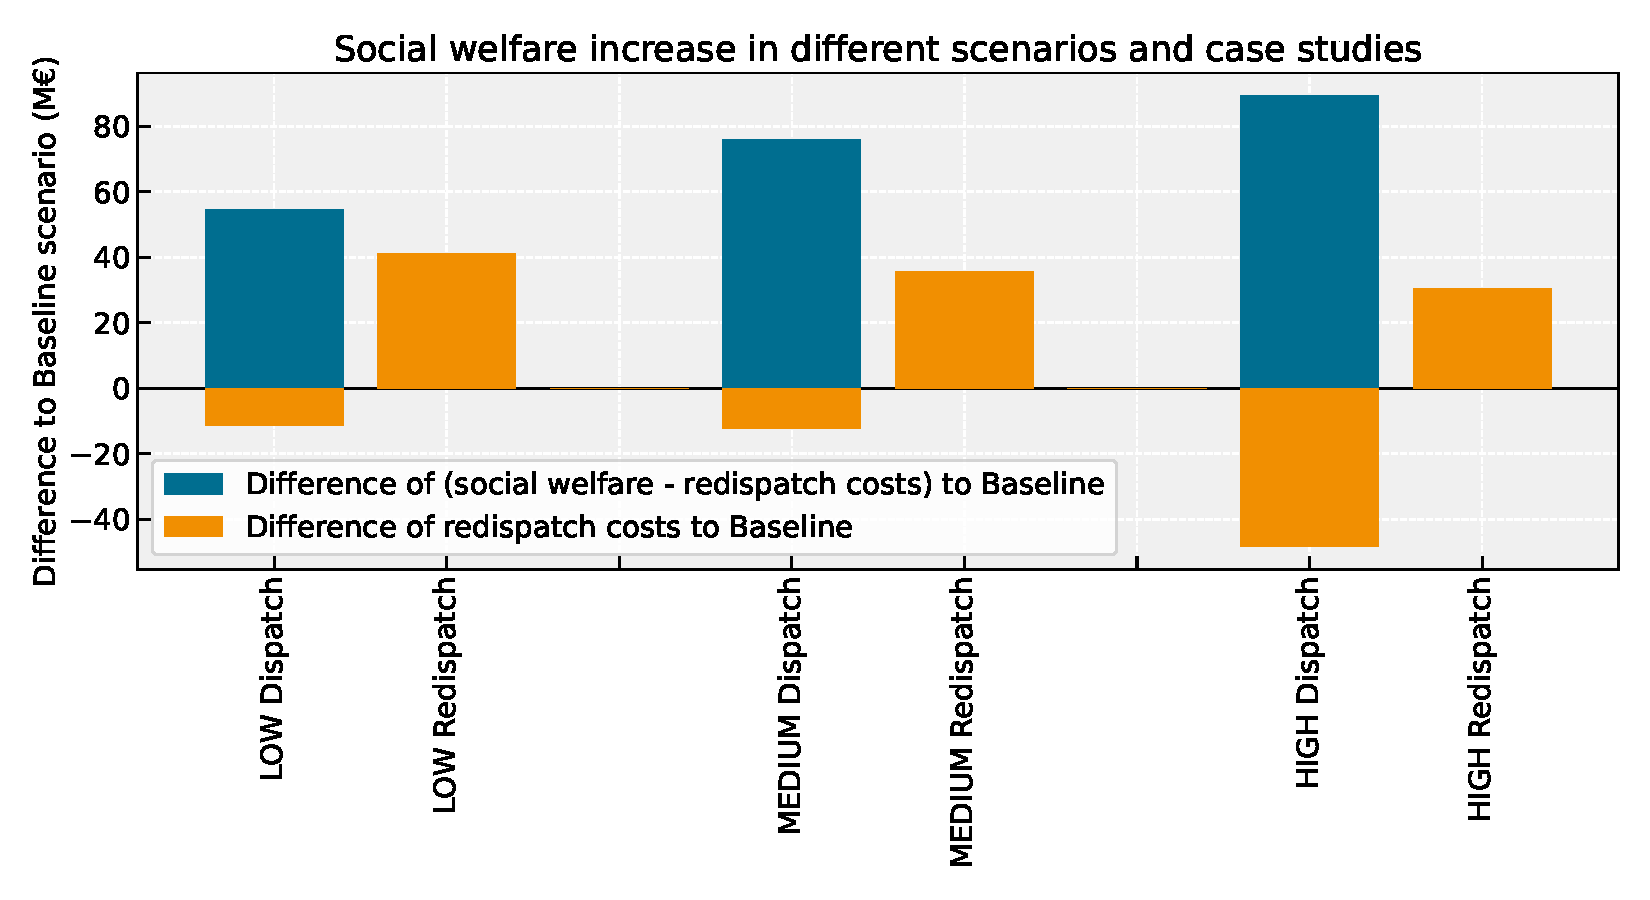
\includegraphics[width=0.9\textwidth]{graphics/appendix_image_costs.pdf}
            \caption{\added{Comparison of using the charging flexibility for dispatch versus for redispatch measures - relative benefits compared to the \textit{Baseline} case.}}
            \label{fig:cost_comp}
        \end{figure}
\added{Figure \ref{fig:cost_comp} displays the difference in the social welfare and the redispatch costs depending on the case studies \textit{Dispatch} and \textit{Redispatch} relative to the \textit{Baseline} scenario for the different electrification scenarios. The social welfare is similar for the \textit{Baseline} and \textit{Redispatch} case. The following two observations are significant here:}

\begin{itemize}
\item \added{The difference between the social welfare minus the redispatch costs (corresponding to the benefit of using charging flexibility for dispatch versus redispatch measures) is steadily increasing with the electrification of the commercial fleet for the \textit{Dispatch} case.}
\item  \added{The relative benefit of allocating the flexibility in the redispatch measures decreases with the rate of electrification in the (\textit{Redispatch} case)}.
\end{itemize}
\added{It is important to note here that this comparison is limited in its informative value concerning benefits of allocating charging flexibility of the commercial fleet in the dispatch or using it of redispatch measures: First, the geographic scope of the two optimizations is significantly different. In the dispatch optimization, the social welfare of the Central European electricity market is maximized, while redispatch costs are minimized exclusively in the Austrian transmission grid. Therefore, the effect on the redispatch costs of the other Central European countries is neglected in this comparison. Second, no costs for the activation of flexibility are considered in both case studies. Third, the absolute risks for system stability and security  in the face of increased requirements for redispatch measures are not accounted for.}
\end{document}

%%
%% End of file `elsarticle-template-num.tex'.
